\documentclass{article}

\usepackage[utf8]{inputenc}
\usepackage[T1]{fontenc}
\usepackage{polski}
\usepackage{indentfirst}
\usepackage{lastpage}
\usepackage{natbib}
\usepackage{graphicx} 
\usepackage{sidecap}
\usepackage{wrapfig}
\usepackage{subfig}
\usepackage{caption}
\usepackage{hyperref}
\usepackage{float}

\usepackage{geometry}
 \geometry{
 a4paper,
 total={170mm,257mm},
 left=20mm,
 top=20mm,
 }

\captionsetup[figure]{name={Zrzut ekranu}}

\usepackage{fancyhdr}
\pagestyle{fancy}
\fancyhf{}
\rhead{Franciszek Wysocki}
\rfoot{Strona \thepage \hspace{1pt} z \pageref{LastPage}}

\title{Sprawozdanie końcowe z realizacji projektu pt. \\ ,,Noticeboard''}
\author{}
\date{}

\begin{document}
\maketitle

\begin{flushright}
\par
\vfill
\par
{\fontsize{11}{11}\selectfont
    Wykonał: Franciszek Wysocki

    Sprawdzający: mgr inż. Paweł Zawadzki

    Data: 04-06-2021
}
\end{flushright}
\thispagestyle{empty}

\newpage
\lhead{Spis treści}
\tableofcontents

\newpage



\lhead{Cel projektu}
\section{Cel projektu}

    Celem projektu było stworzenie serwisu ogłoszeniowego - aplikacji webowej w architekturze klient-serwer, która umożliwi m.in. rejestrację i logowanie, wyświetlanie, dodawanie, edytowanie i kasowanie pojedyńczych ogłoszeń  oraz pobieranie (paginacja, lazy loading), sortowanie i filtrowanie stron z ogłoszeniami.

\section{Wykorzystane technologie}
    Baza danych:
    \begin{itemize}
        \item PostGreSQL;
        \item Docker.
    \end{itemize}
    
    Back-end:
    \begin{itemize}
        \item Java;
        \item Spring Boot.
    \end{itemize}
    
    Front-end:
        \begin{itemize}
        \item JavaScript;
        \item React;
        \item Redux;
        \item Bootstrap 5;
        \item Css;
        \item Html.
    \end{itemize}
    Wersje zostały wymienione  w specyfikacji implementacyjnej.
    
\section{Zmiany względem specyfikacji}
    Zaplanowana struktura projektu, wykorzystane narzędzia oraz sposoby testowania nie zmieniły się znacząco względem założeń. \\
    
    Zmianie uległo natomiast kilka funkcjonalności: dodanie profilu użytkownika, dodanie możliwości zmiany hasła, możliwości skasowania konta, aktywację konta poprzez e-mail. \\

    Z podstawowych założeń, które zakładałem nie implementowałem jedynie podziału na kategorie (uznałem to za zbędne i wolałem skupić się na innych dodatkowych funkcjach).
\section{Uruchomienie aplikacji}
    Aplikacja w wersji produkcyjnej jest uruchomiona na stałe i można z niej korzystać pod adresem \\ \href{https://noticeboard.pl}{https://noticeboard.pl}. \\
    Aplikację starałem się zrobić możliwie bezpieczną (hashowane hasła użytkownika, szyfrowane hasła do bazy danych, maila itd... w pliku application.yml, szyfrowane połączenie HTTPS), jednak wolałbym nie odpowiadać za pozostawione tam dane, dlatego polecam skorzystać z \href{https://temp-mail.org/en/}{tymczasowego adresu e-mail}, \href{https://random-data-generator.com/generator-losowych-imion-i-nazwisk/}{generatora imion i nazwisk} oraz \href{https://thispersondoesnotexist.com/}{generatora twarzy}, a do samych treści ogłoszeń np. \href{https://olx.pl}{z innego serwisu ogłoszeniowego}.\\
    
    Aby uruchomić aplikację w trybie deweloperskim należy oddzielnie uruchomić (1) serwer z bazą danych, (2) back-end i (3) front-end.
\begin{enumerate}
    \item Uruchomienie serwera bazy danych PostgreSQL w dockerze (port: 5555):\\
    \texttt{docker-compose up database}\\
    \item Uruchomienie aplikacji back-endowej (port: 8080):\\
    Aby utworzyć plik wykonywalny można wykorzystać Mavena: \\
    \texttt{mvn clean install} \\
    a następnie: \\
    \texttt{java -Djasypt.encryptor.password=secretKey -jar noticeboard-0.0.1-SNAPSHOT.jar} \\
    W miejsce secretKey należy podać klucz umożliwiający odszyfrowanie haseł do bazy danych, skrzynki mailowej oraz magazynu na klucze (SSL), znajdujących się w pliku application.yml. \\
    \item Uruchomienie aplikacji front-endowej (port: 3000):\\
    Tutaj również na początku należy skorzystać z menadżera pakietów (zewnętrzne pakiety nie są przechowywane w repozytorium): \\
    \texttt{npm install} \\
    a następnie można uruchomić aplikację:\\
    \texttt{npm start}\\
\end{enumerate}
    Testy można uruchomić niezależnie (nie wymagają one podania klucza):
    \begin{enumerate}
        \item Back-end: \\
        \texttt{mvn test} \\
        \item Front-end: \\
        \texttt{npm test} \\
    \end{enumerate}

\lhead{Przykładowe scenariusze użytkowania}
\section{Przykładowe scenariusze użytkowania}
\begin{itemize}
    \item Użytkownik jest ogłoszeniobiorcą.
        \begin{enumerate}
            \item Użytkownik przechodzi pod wskazany adres URL  \href{https://noticeboard.pl}{https://noticeboard.pl} i bez zalogowania może przeglądać strony z ogłoszeniami.
                \begin{center}
                
                 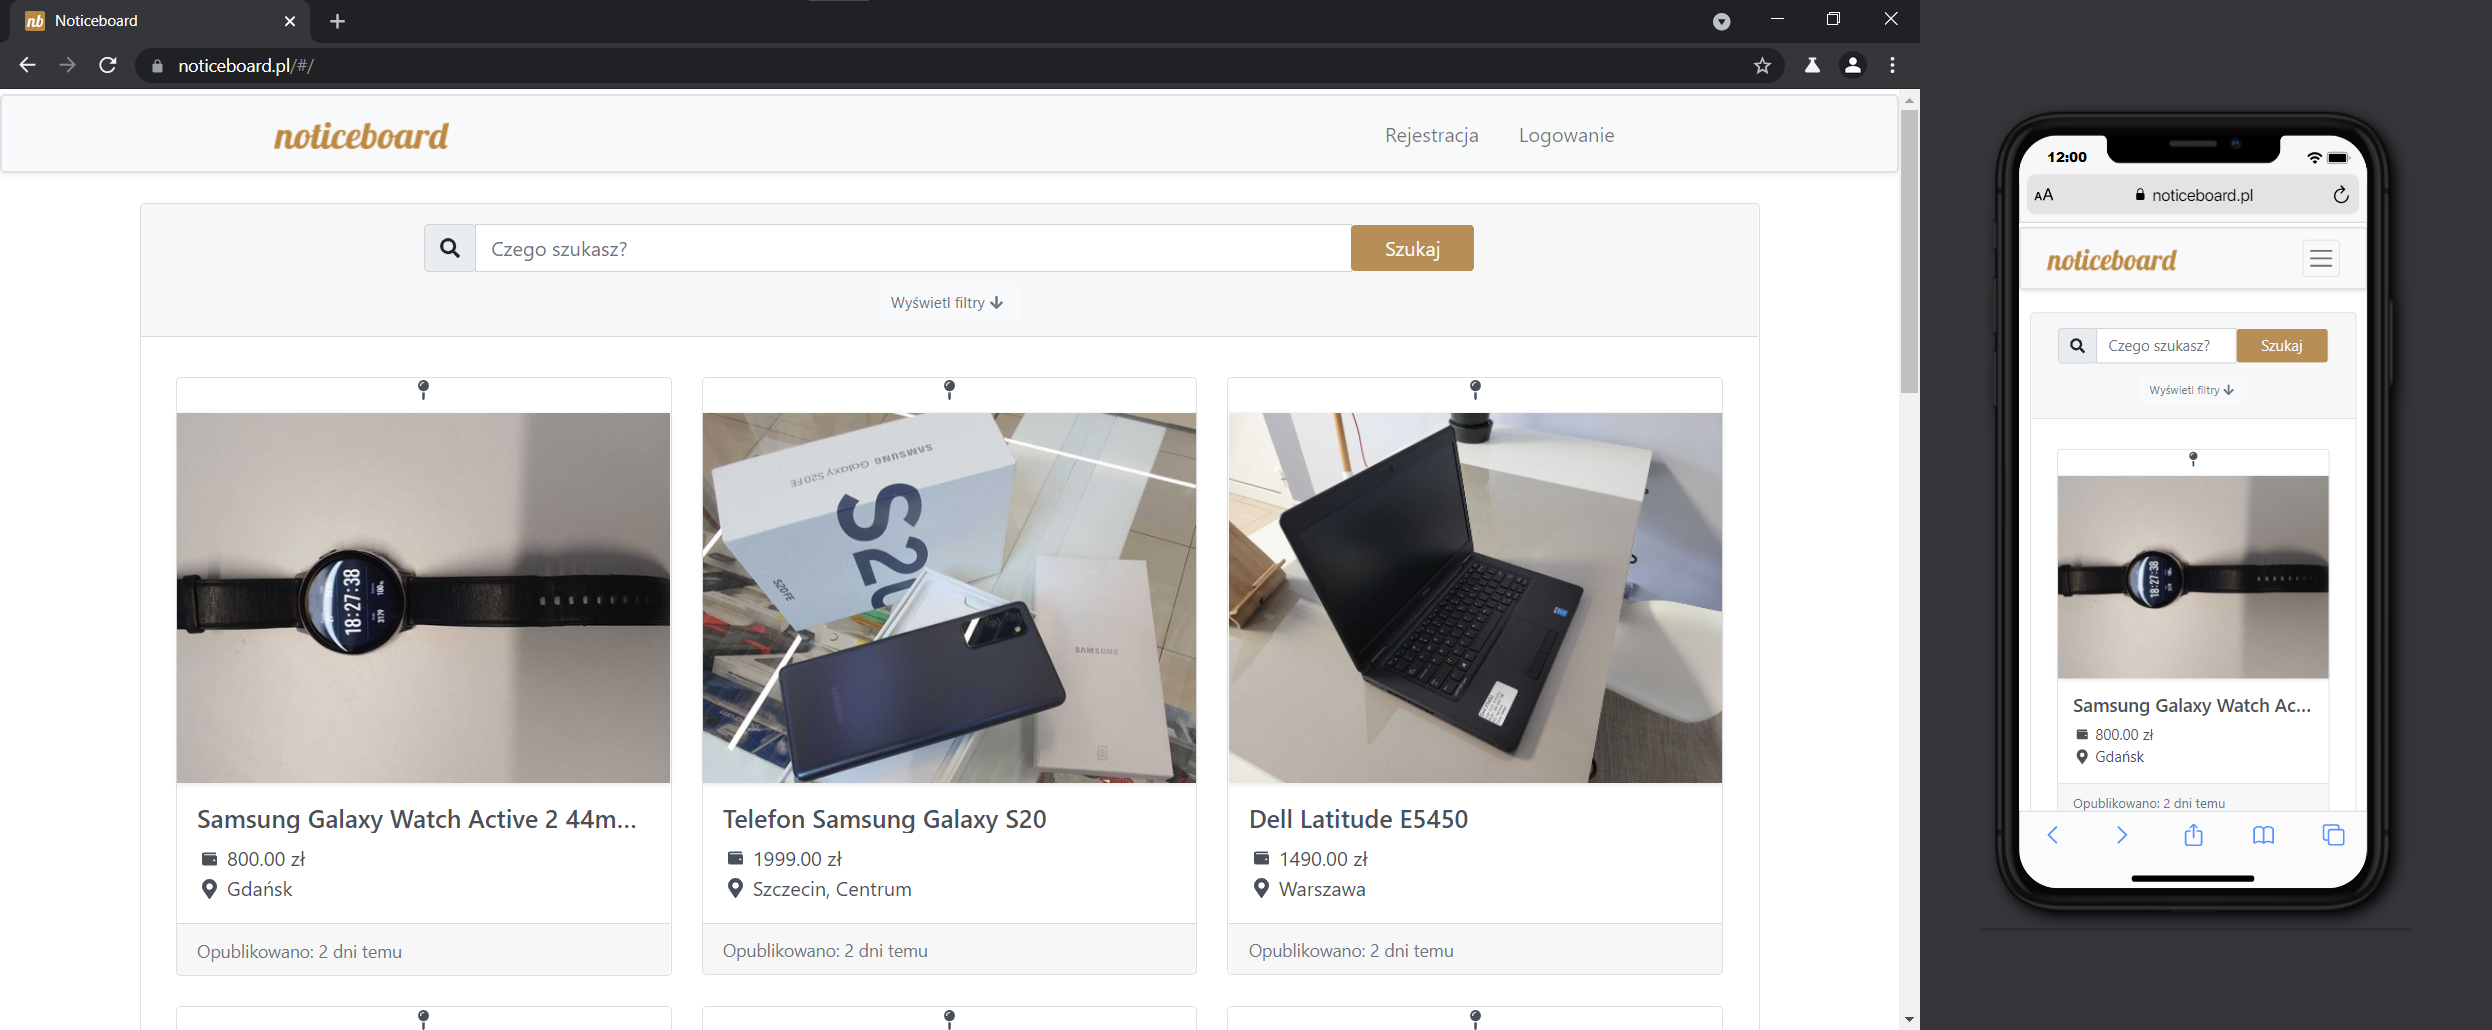
\includegraphics[width=15.5cm]{StronaGłówna.png}
                    \captionof{figure}{}
                \end{center}
            \item Użytkownik filtruje i sortuje ogłoszenia.
            \begin{center}
                    \centering  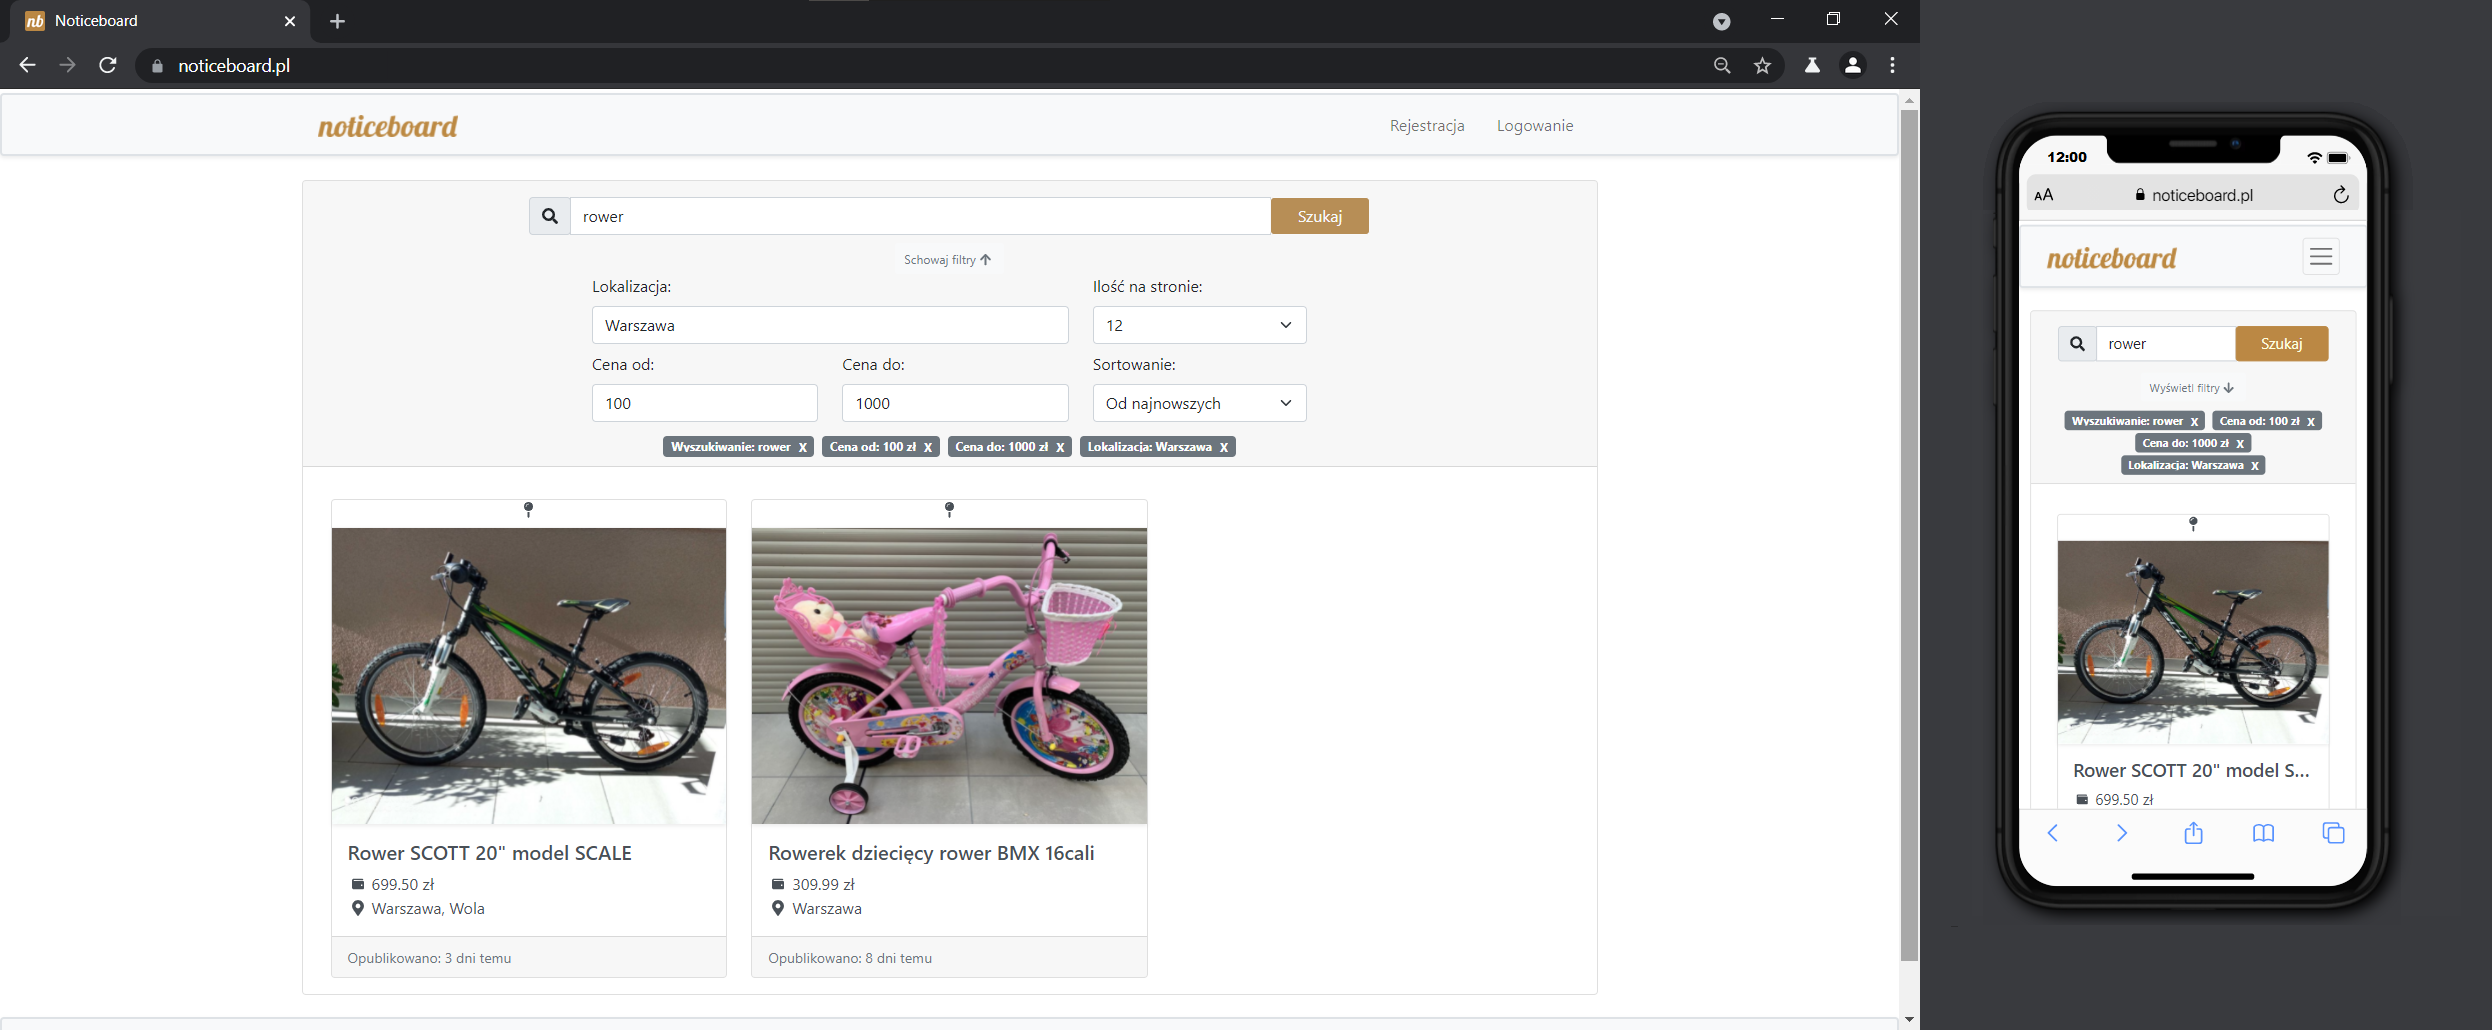
\includegraphics[width=15.5cm]{Filtrowanie.png}
                   \captionof{figure}{}
                \end{center}
            \item Użytkownik otwiera ogłoszenie i wyświetla szczegółowy opis, dane sprzedawcy i jego adres email do kontaktu.
            \begin{center}
                    \centering  \includegraphics[width=15.5cm]{StronaOgłoszenia.png}
                   \captionof{figure}{}
            \end{center}
            \item Użytkownik przechodzi na stronę (w tym przypadku innego) sprzedawcy i przegląda jego inne ogłoszenia.
            \begin{center}
                    \centering  \includegraphics[width=15.5cm]{StronaUżytkownika.png}
                   \captionof{figure}{}
            \end{center}
        \end{enumerate}
        
    \item Użytkownik zakłada konto oraz loguje się:
        \begin{enumerate}
            \item Użytkownik przechodzi na stronę rejestracji i wprowadza wymagane dane.
            \begin{center}
                    \centering  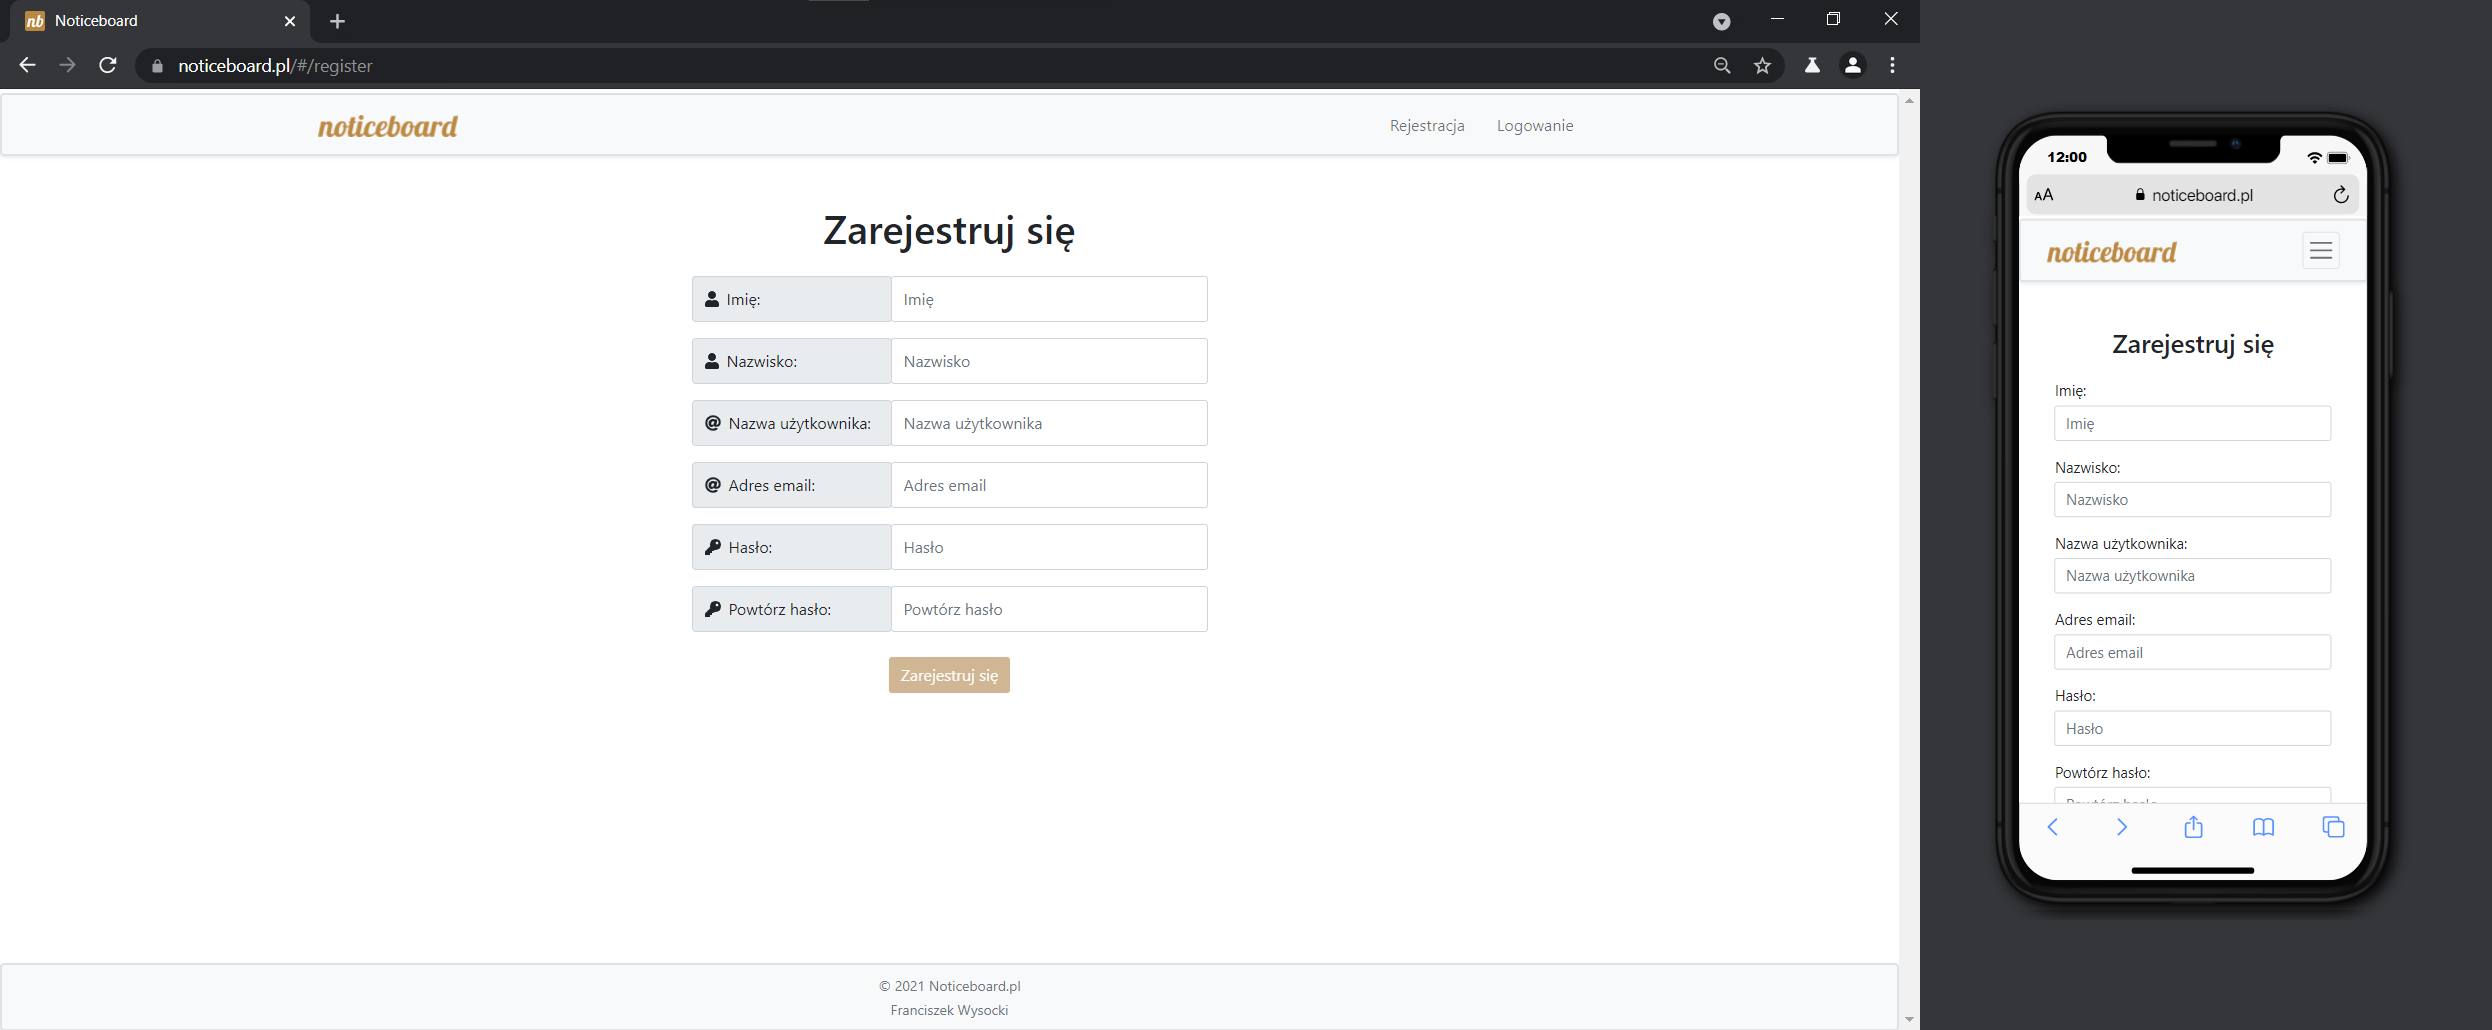
\includegraphics[width=15.5cm]{StronaRejestracji.png}
                   \captionof{figure}{}
            \end{center}
            \item Użytkownik zostaje poinformowany o wysłaniu maila z linkiem aktywacyjnym.
            \begin{center}
                    \centering  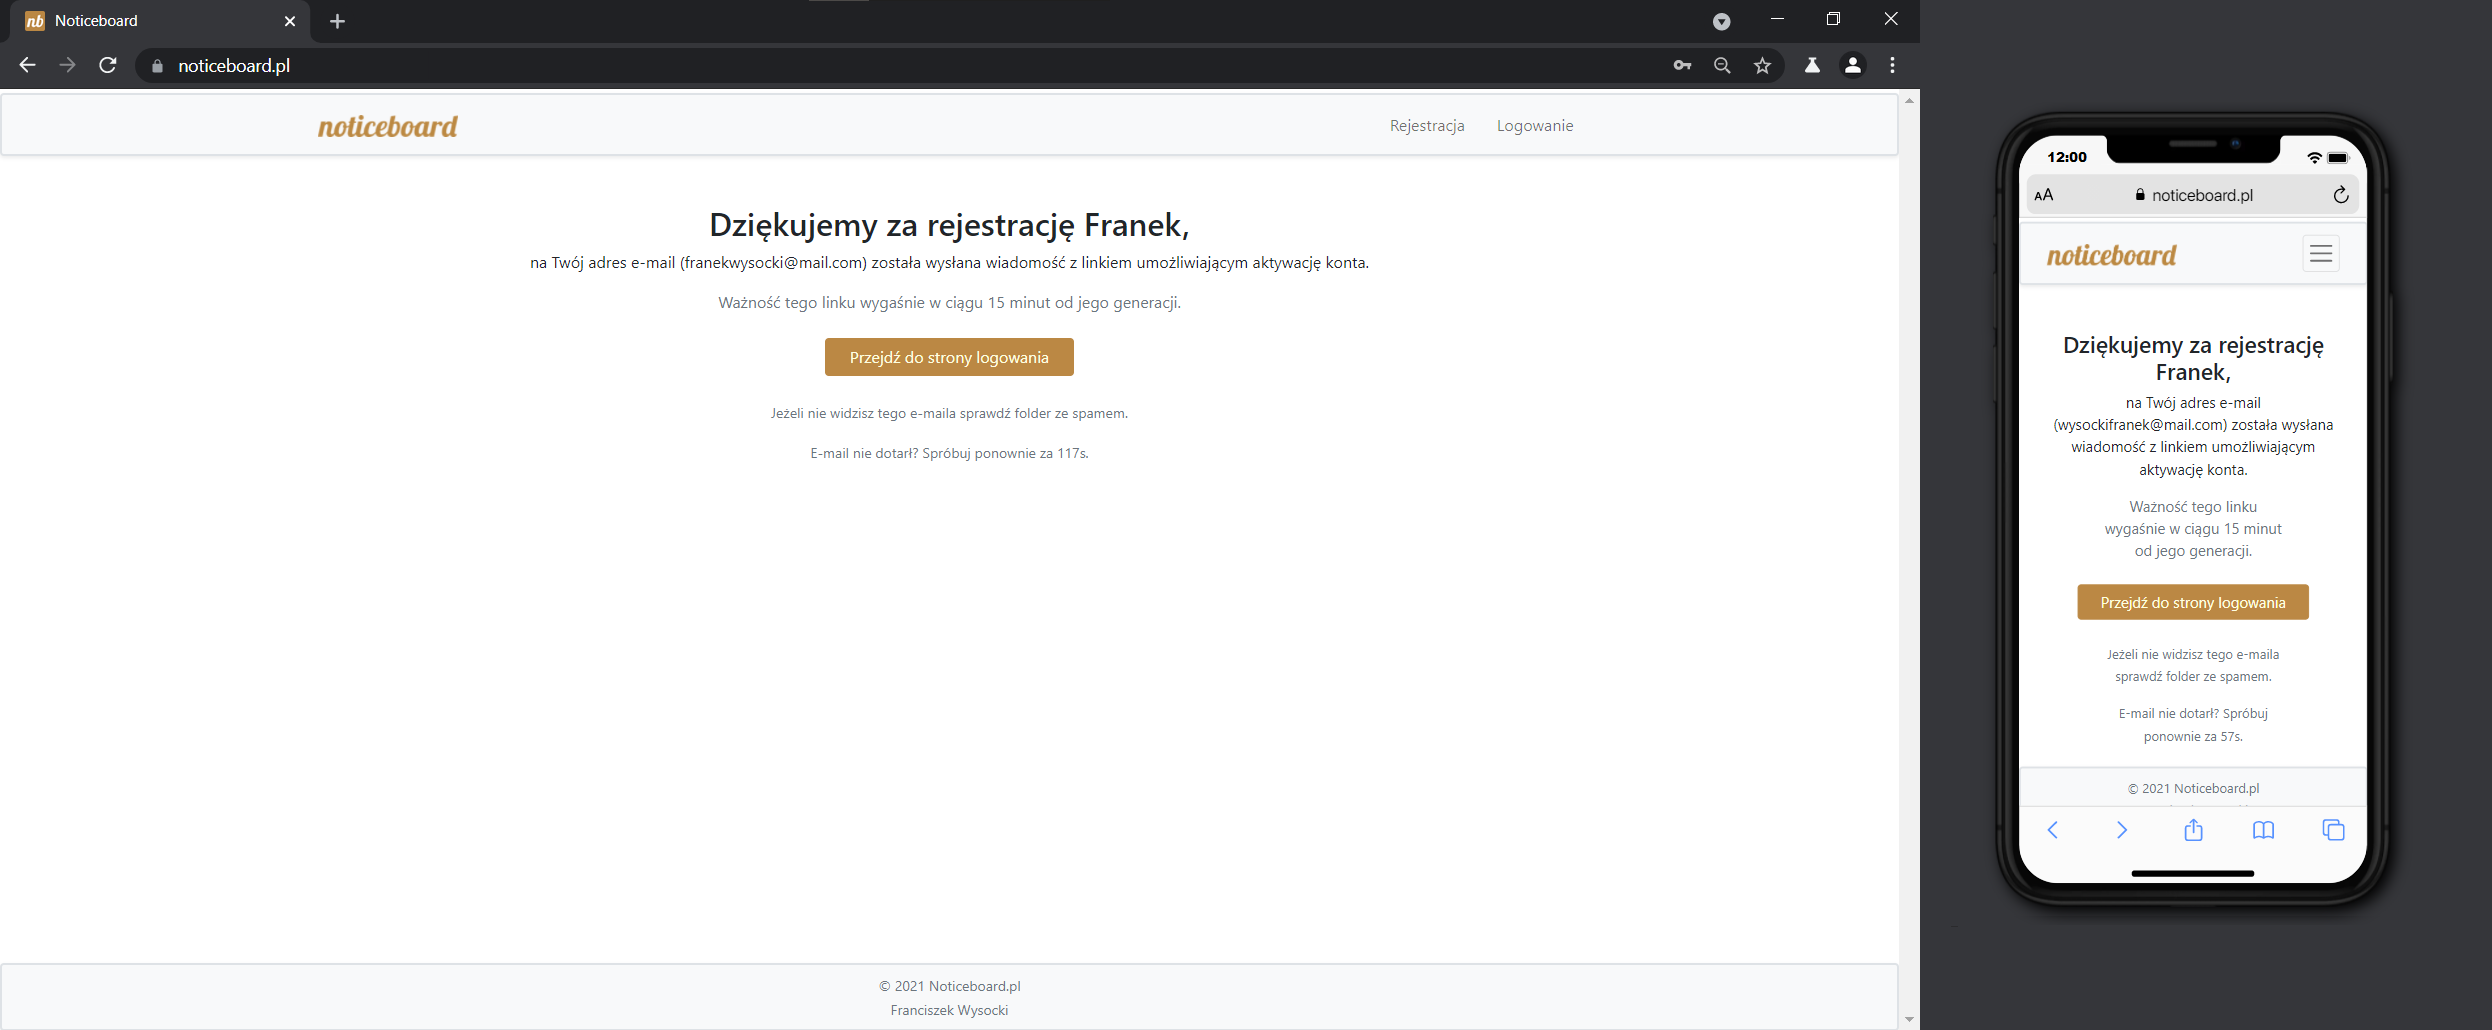
\includegraphics[width=15.5cm]{StronaPotwierdzeniaRejestracji.png}
                   \captionof{figure}{}
            \end{center}
            \item Użytkownik otwiera skrzynkę mailową i klika w link aktywacyjny.
            \begin{center}
                    \centering  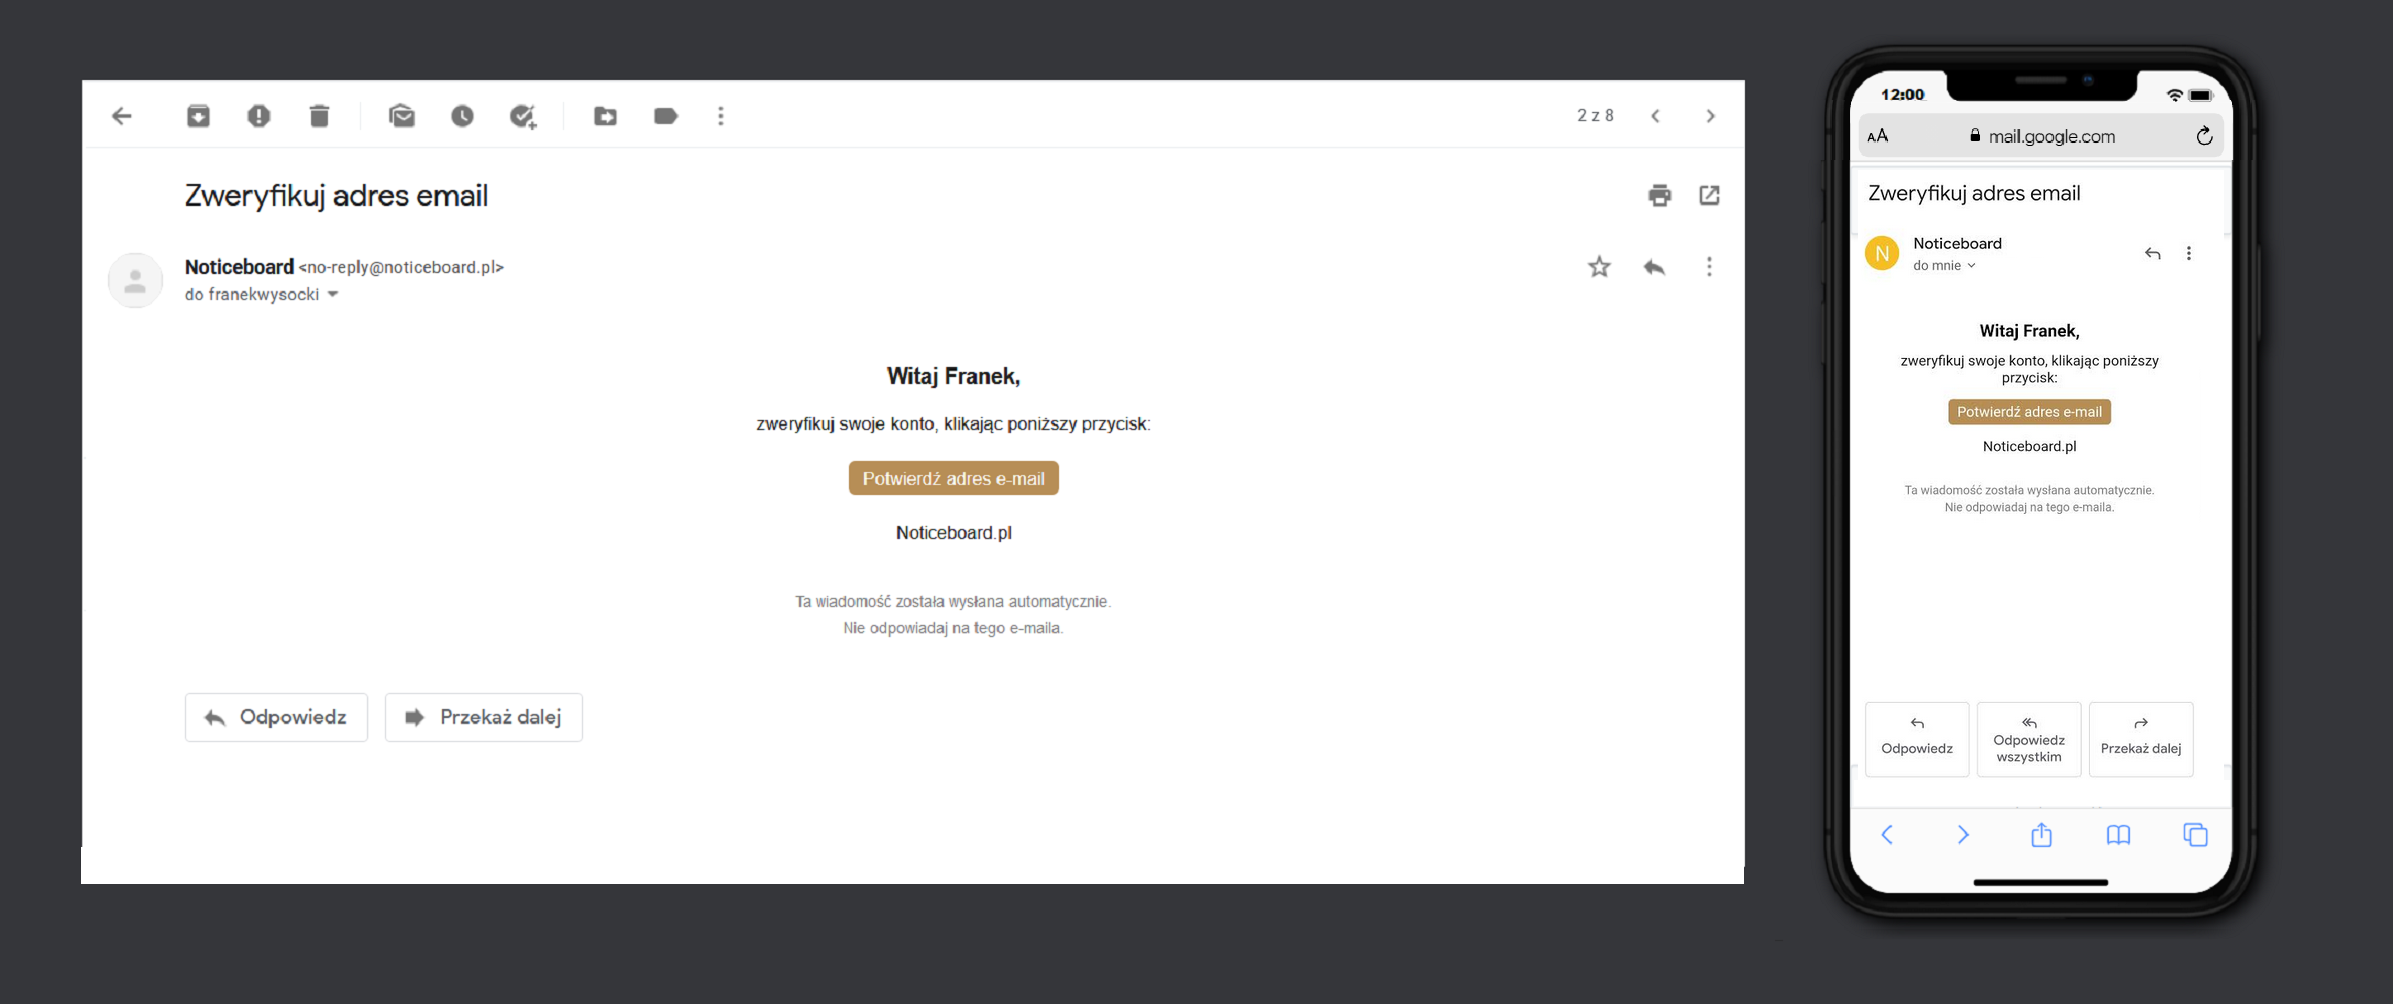
\includegraphics[width=15.5cm]{Mail.png}
                   \captionof{figure}{}
            \end{center}
            \item Użytkownik zostaje poinformowany o sukcesie operacji i ma możliwość przejścia do strony logowania.
            \begin{center}
                    \centering  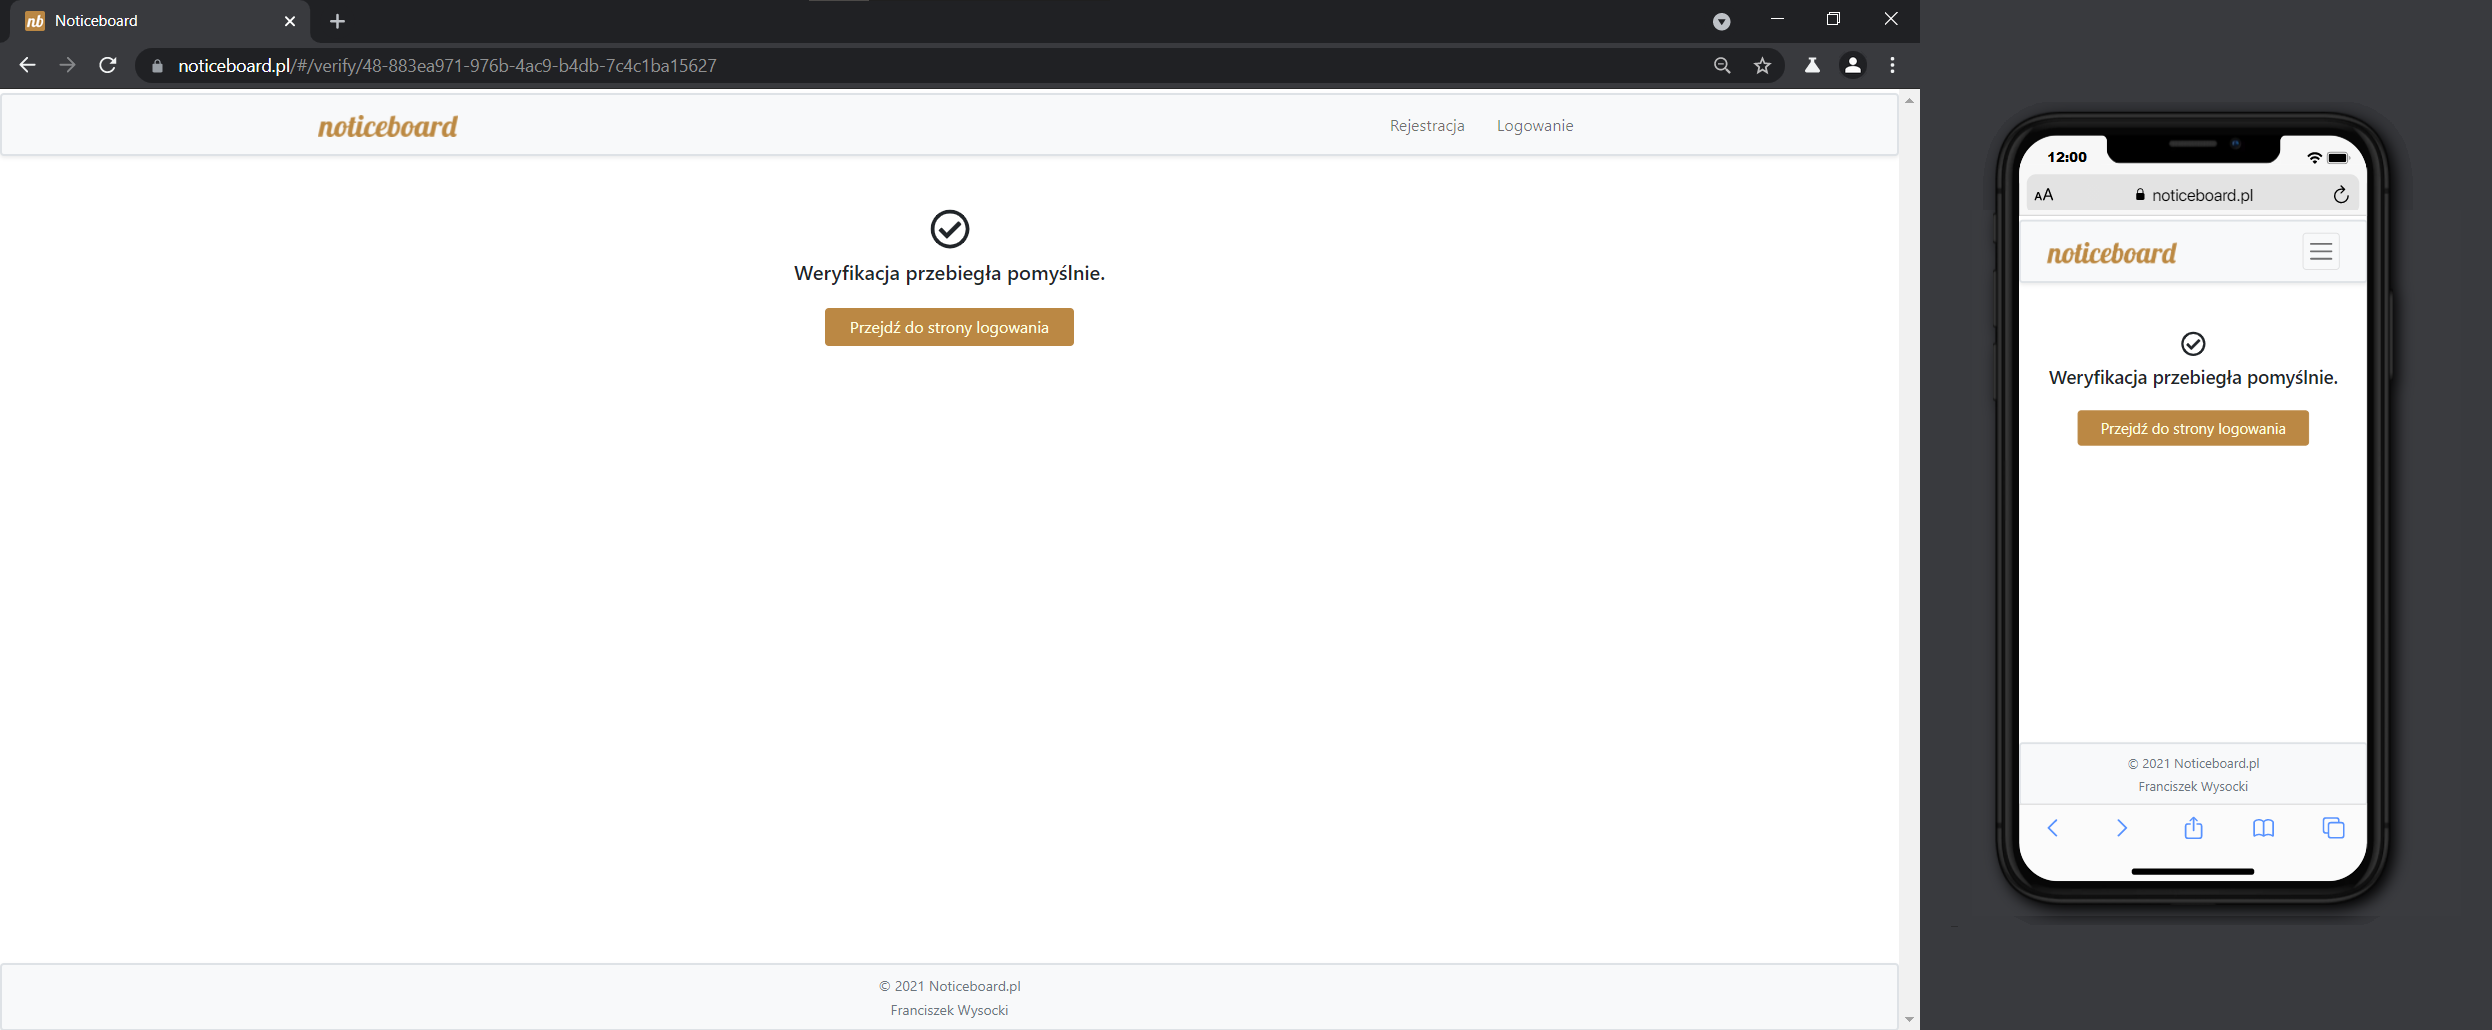
\includegraphics[width=15.5cm]{Weryfikacja.png}
                   \captionof{figure}{}
            \end{center}
            \item Użytkownik loguje się.
            \begin{center}
                    \centering  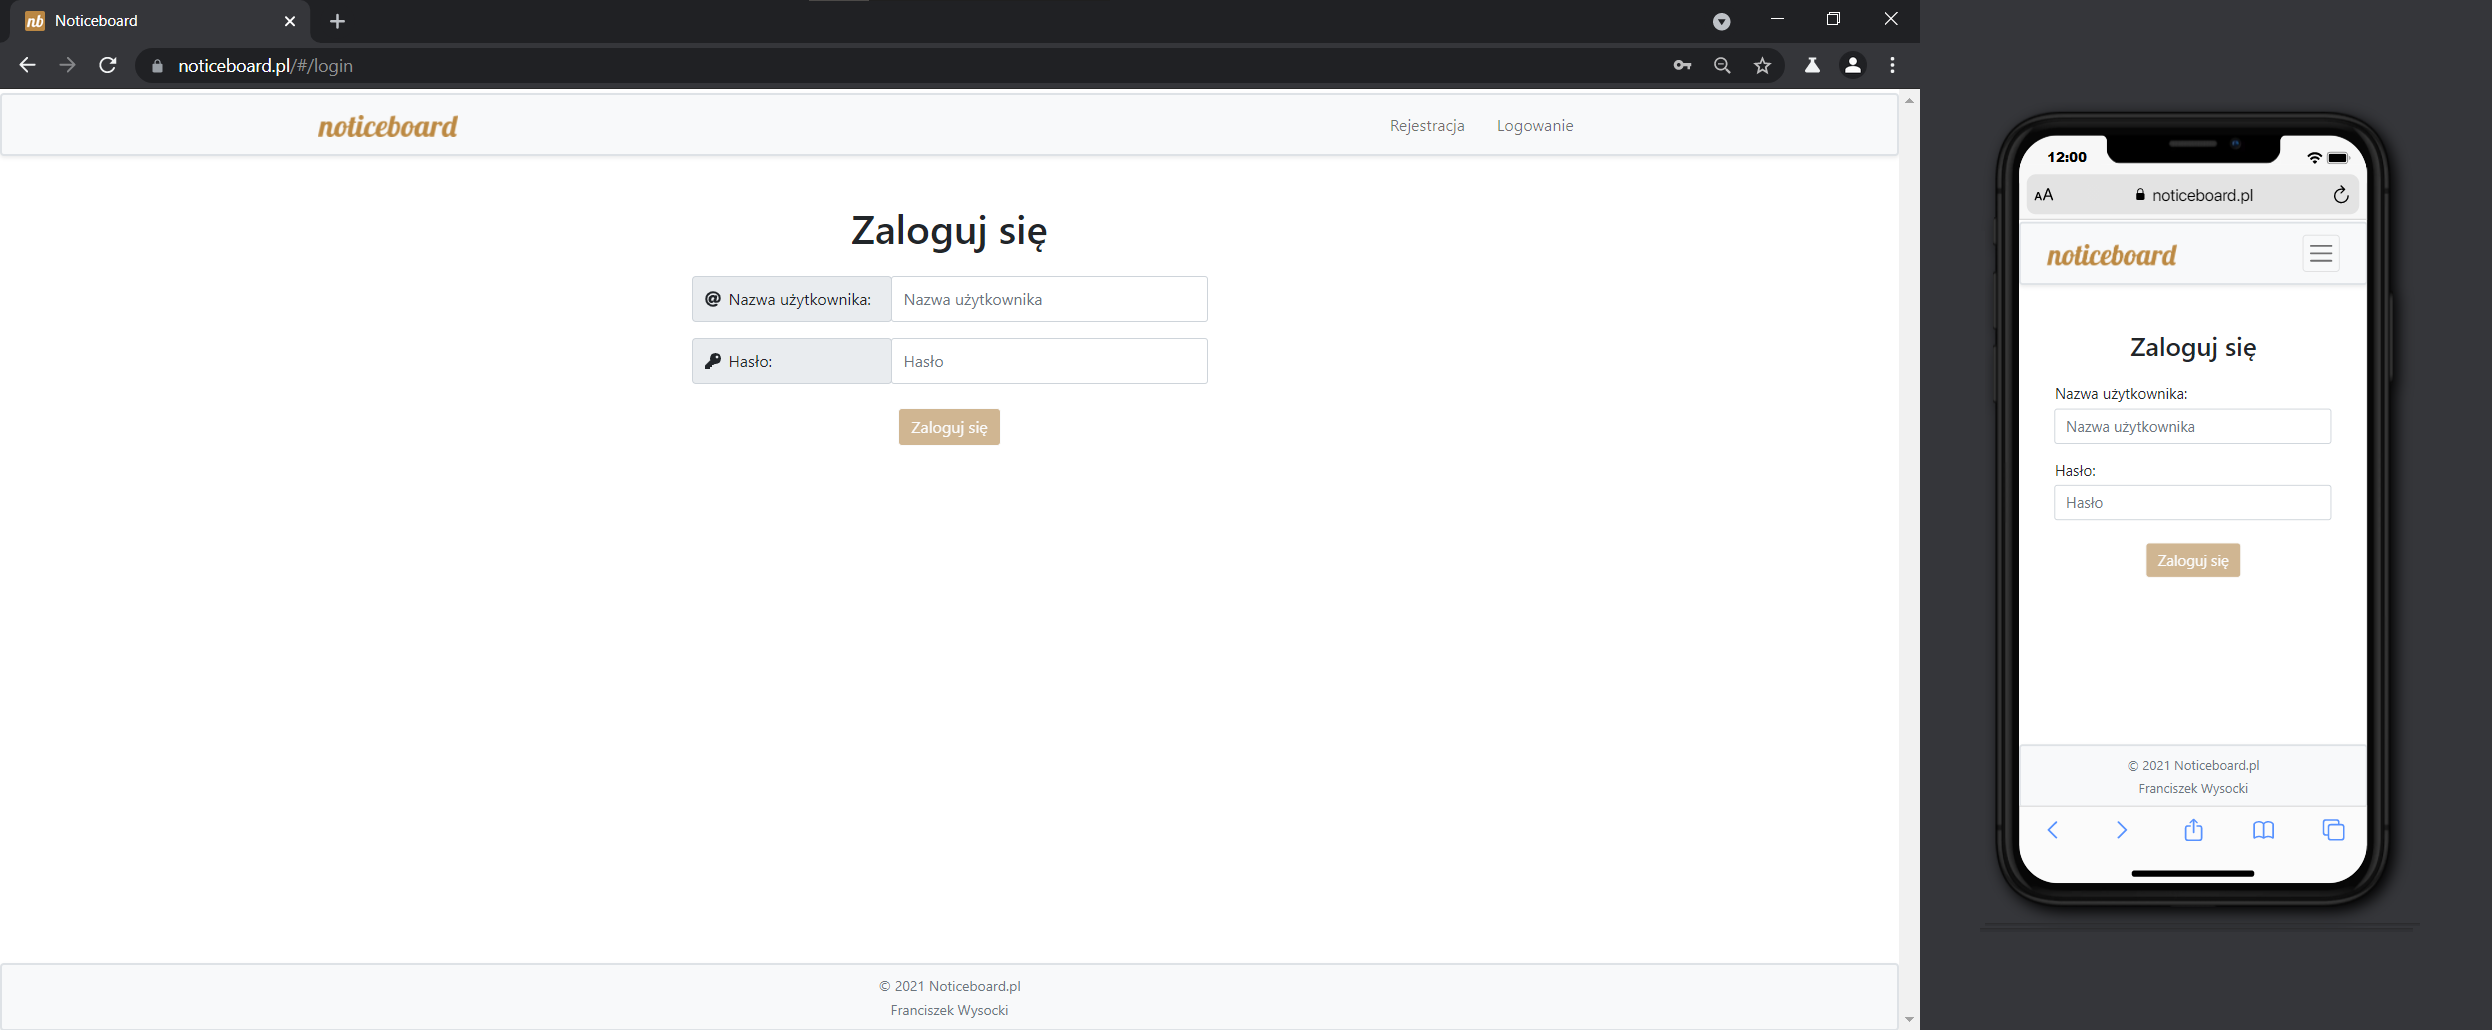
\includegraphics[width=15.5cm]{StronaLogowania.png}
                   \captionof{figure}{}
            \end{center}
            \item Użytkownik zostaje przekierowany na stronę główną.
        \end{enumerate}
        
    \item Użytkownik zarządza swoim kontem
        \begin{enumerate}
            \item Zalogowany użytkownik przechodzi na swój profil. Jedynie on ma możliwość wyświetlenia panelu edycji. Użytkownik w samym panelu może zmienić zdjęcie profilowe, imię oraz nazwisko.
            \begin{center}
                    \centering  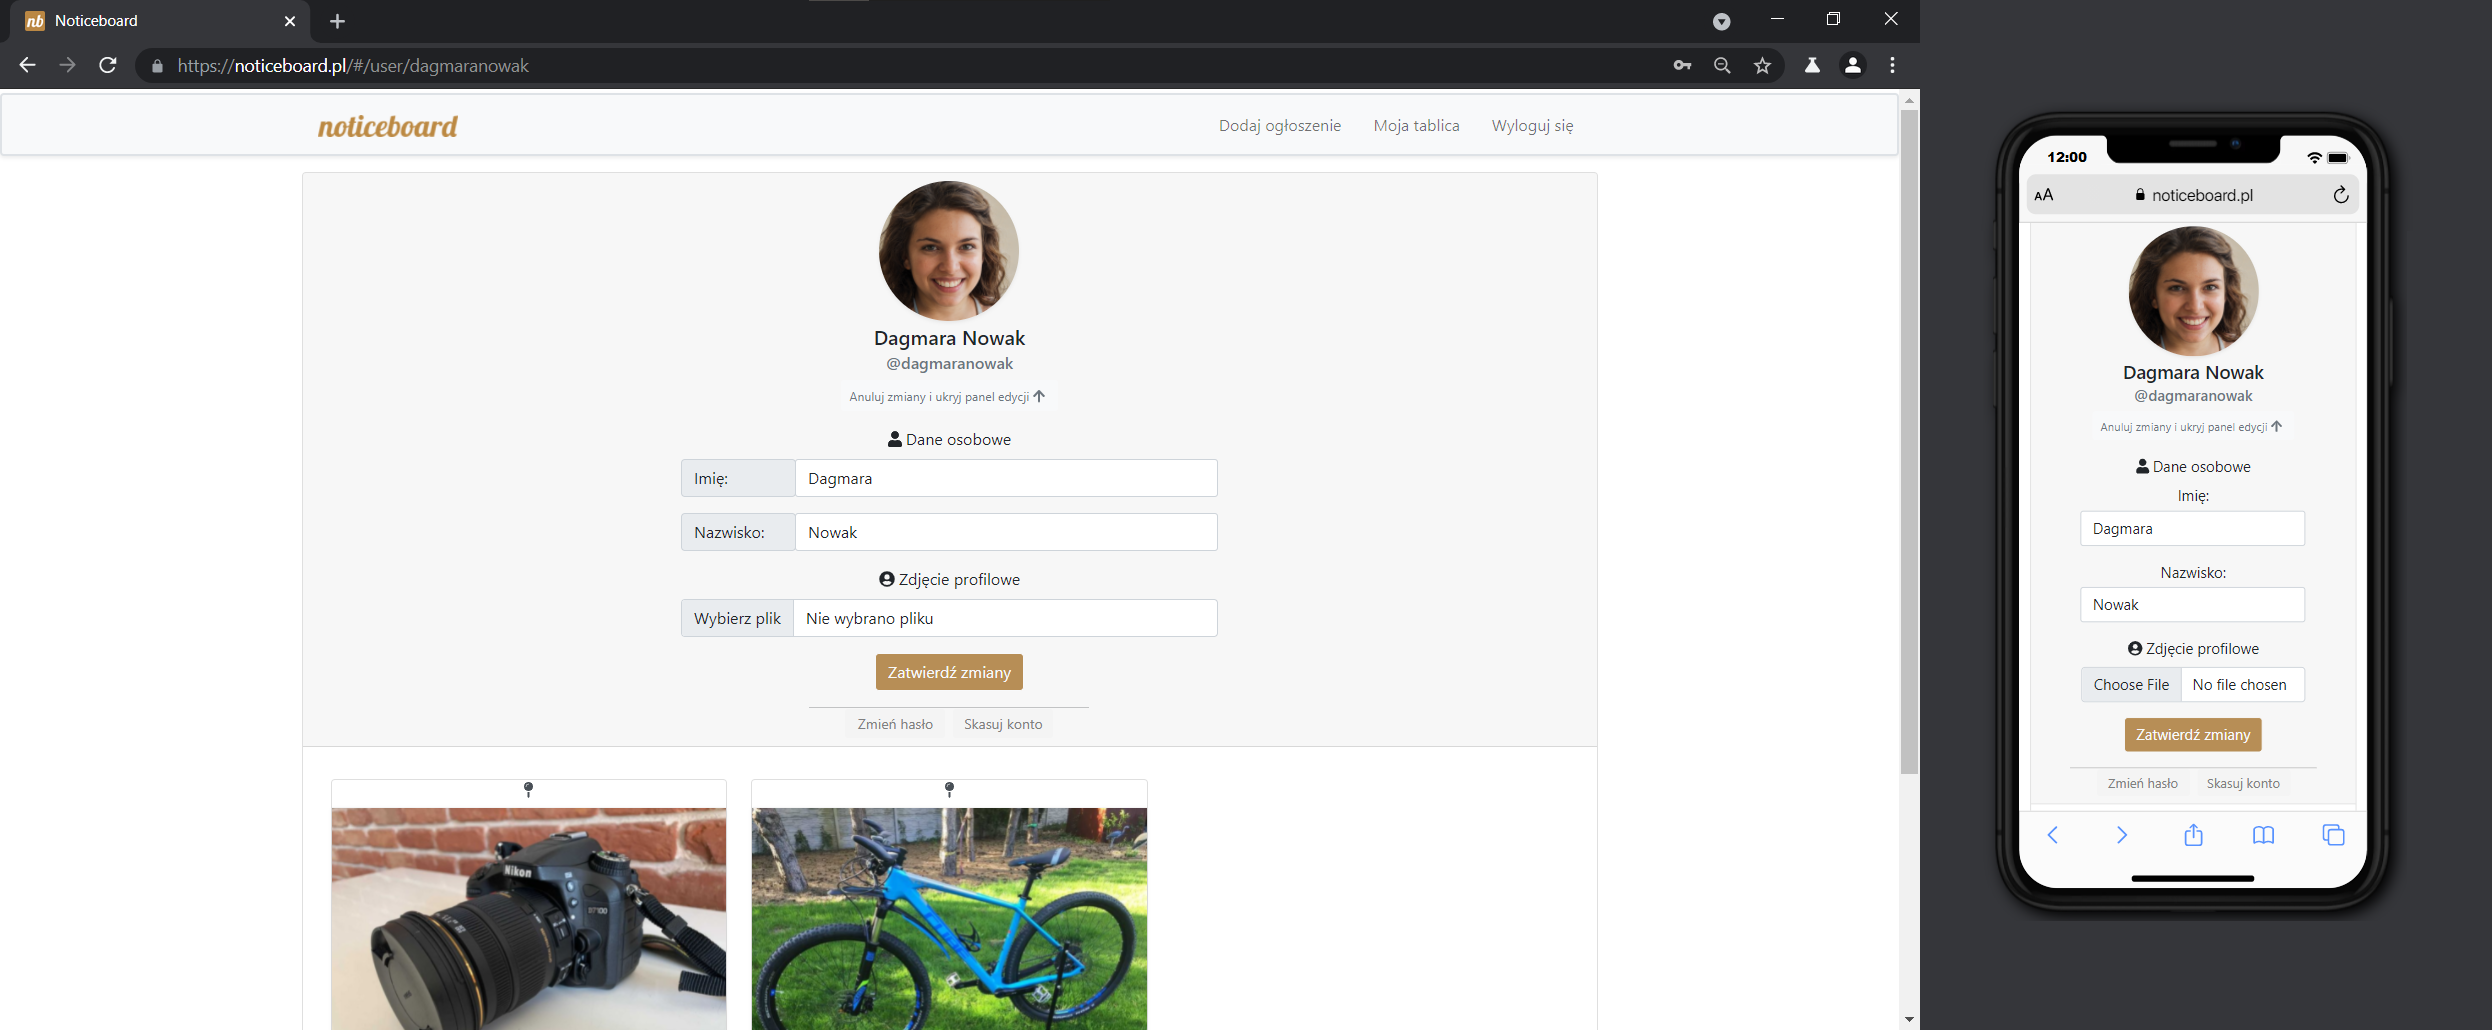
\includegraphics[width=15.5cm]{StronaUżytkownikaWłaściciel.png}
                   \captionof{figure}{}
            \end{center}
            \item Użytkownik kilka ,,Zmień hasło''.
            \begin{center}
                    \centering  \includegraphics[width=15.5cm]{ZmianaHasła.png}
                   \captionof{figure}{}
            \end{center}
            \item Użytkownik kilka ,,Skasuj konto''.
            \begin{center}
                    \centering  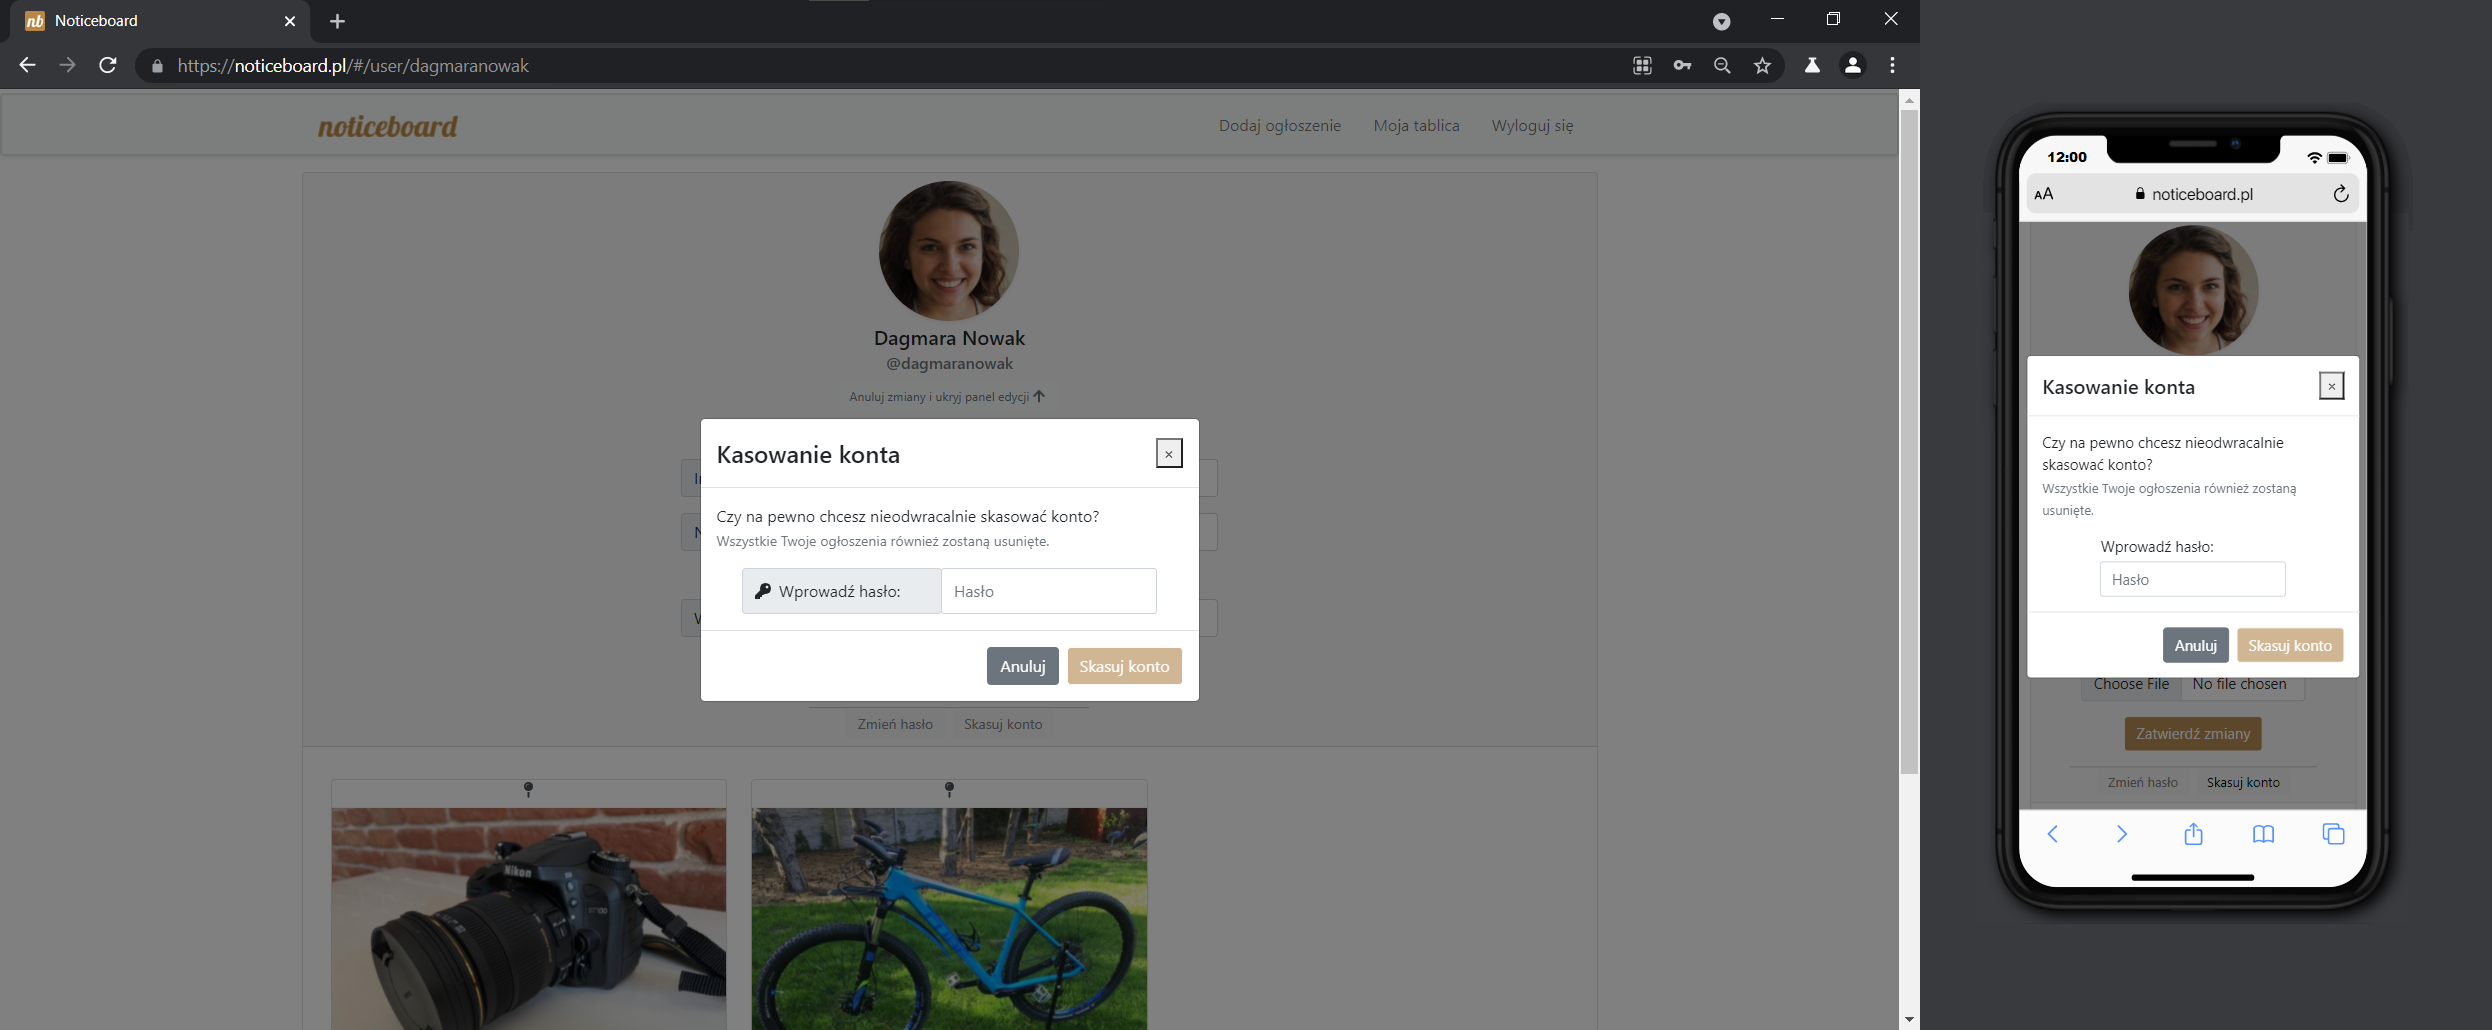
\includegraphics[width=15.5cm]{KasowanieKonta.png}
                   \captionof{figure}{}
            \end{center}
        \end{enumerate}

    \item Użytkownik jest ogłoszeniodawcą.
            \begin{enumerate}
            \item Zalogowany użytkownik klika ,,Dodaj ogłoszenie'' na pasku nawigacyjnym.
            \item Użytkownik podaje tytuł, opis, cenę, lokalizację, adres email oraz załadowuje zdjęcia, po czym zatwierdza operację.
            \begin{center}
                    \centering  \includegraphics[width=15.5cm]{DodanieOgłoszenia.png}
                   \captionof{figure}{}
            \end{center}
            \item Użytkownik przechodzi na stronę swojego ogłoszenia (zamiast linku do jego profilu ma przyciski do skasowania i edycji ogłoszenia).
            \begin{center}
                    \centering  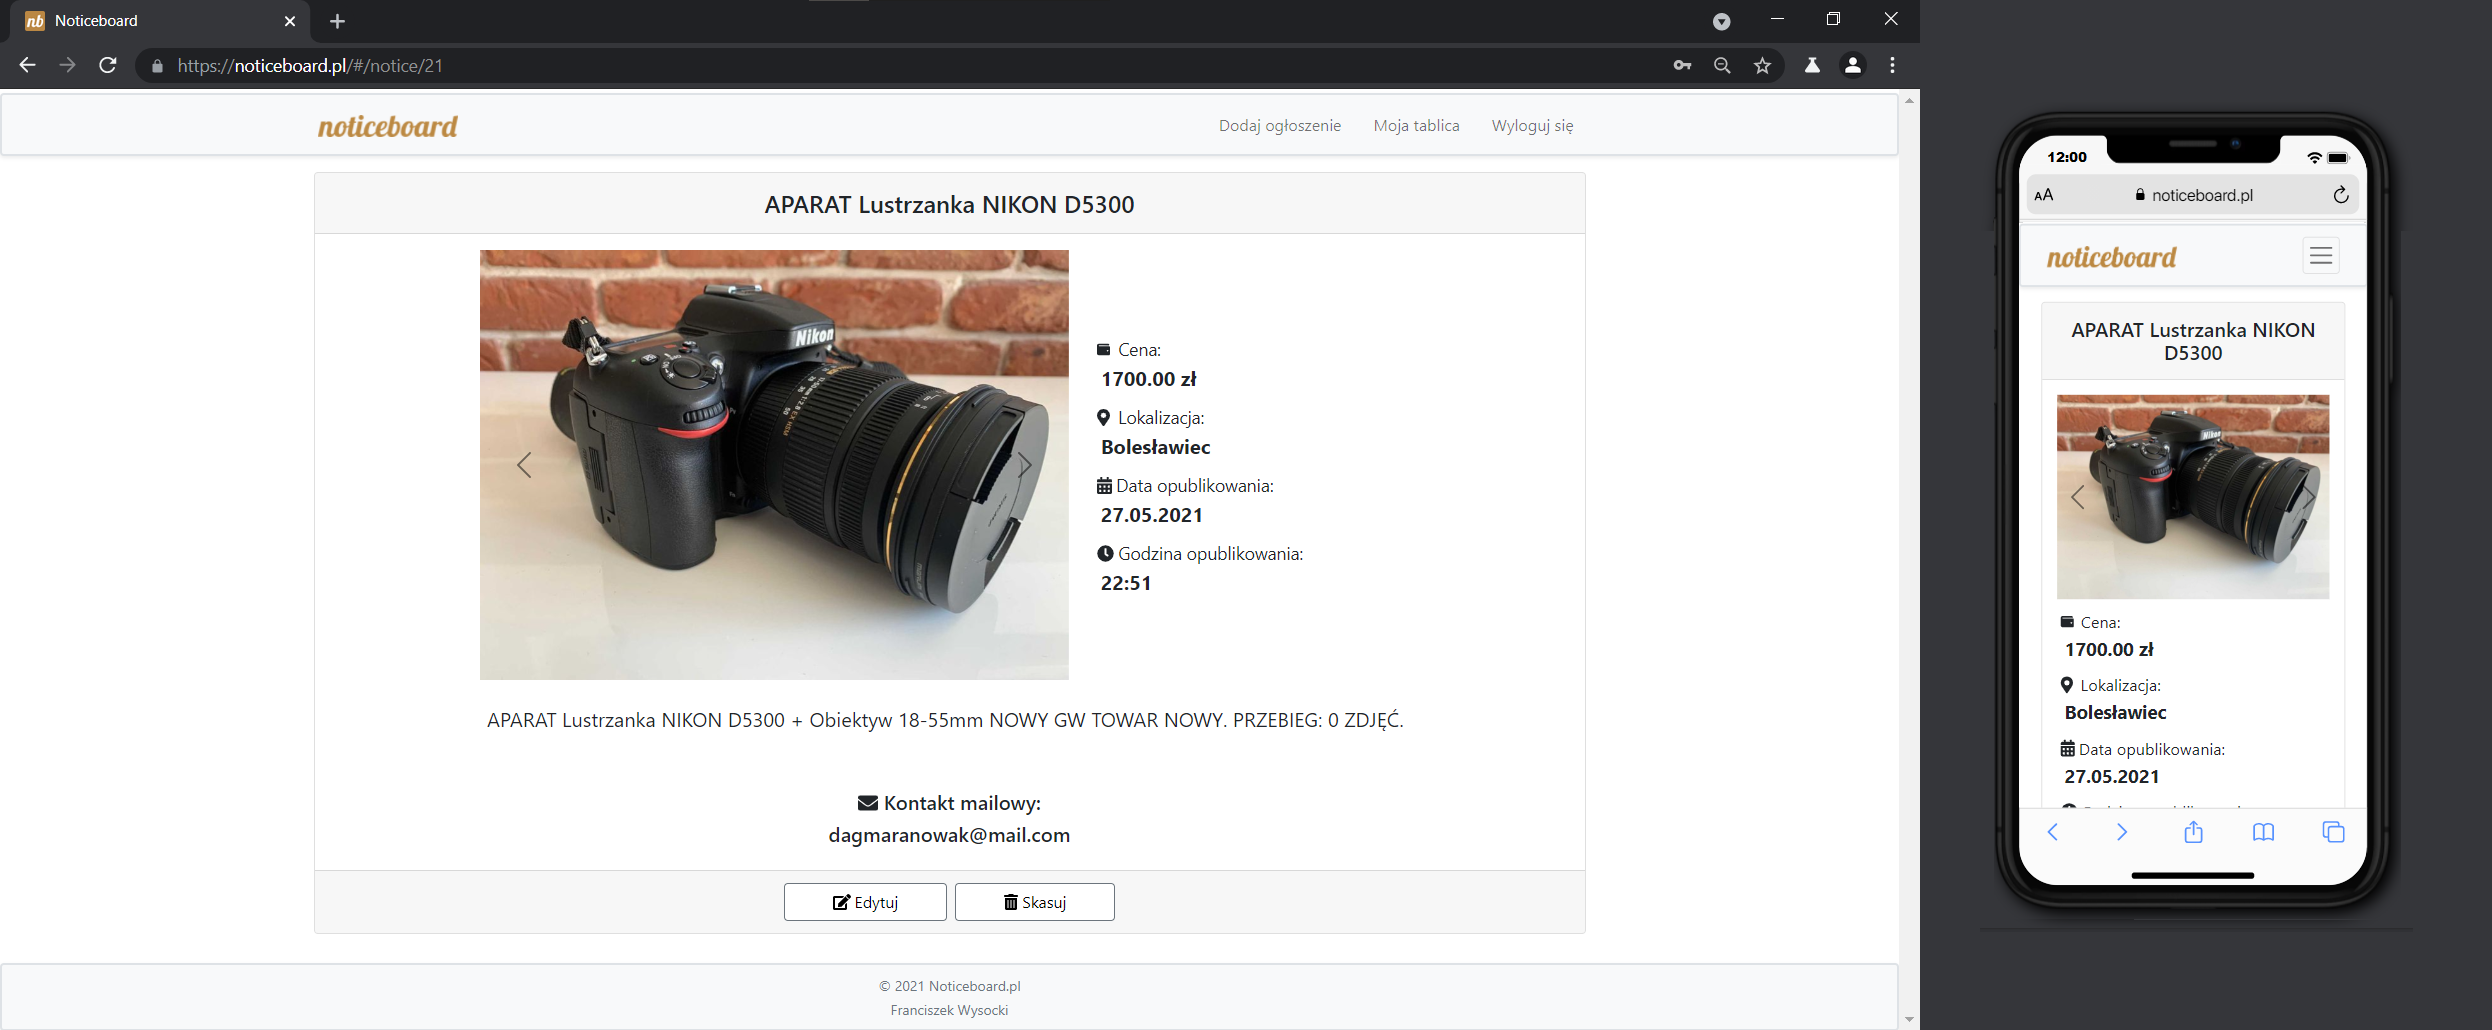
\includegraphics[width=15.5cm]{StronaOgłoszeniaWłaściciel.png}
                   \captionof{figure}{}
            \end{center}
            \item Użytkownik edytuje swoje (np. błędne) ogłoszenie.
            \begin{center}
                 \includegraphics[width=15.5cm]{EdycjaOgłoszenia.png}
                   \captionof{figure}{}
            \end{center}
            \item Użytkownik kasuje swoje (np. nieaktualne) ogłoszenie.
            \begin{center}
                    \centering  \includegraphics[width=15.5cm]{KasowanieOgłoszenia.png}
                   \captionof{figure}{}
            \end{center}
            \item Użytkownik wylogowuje się i zostaje przekierowany na stronę główną.
        \end{enumerate}
    \end{itemize}

    \lhead{Reakcje na błędy ze strony użytkownika}
    \section{Reakcje na błędy ze strony użytkownika}
    \begin{itemize}
        \item Użytkownik przechodzi pod niepoprawny adres URL:
                    \begin{center}
                    \centering  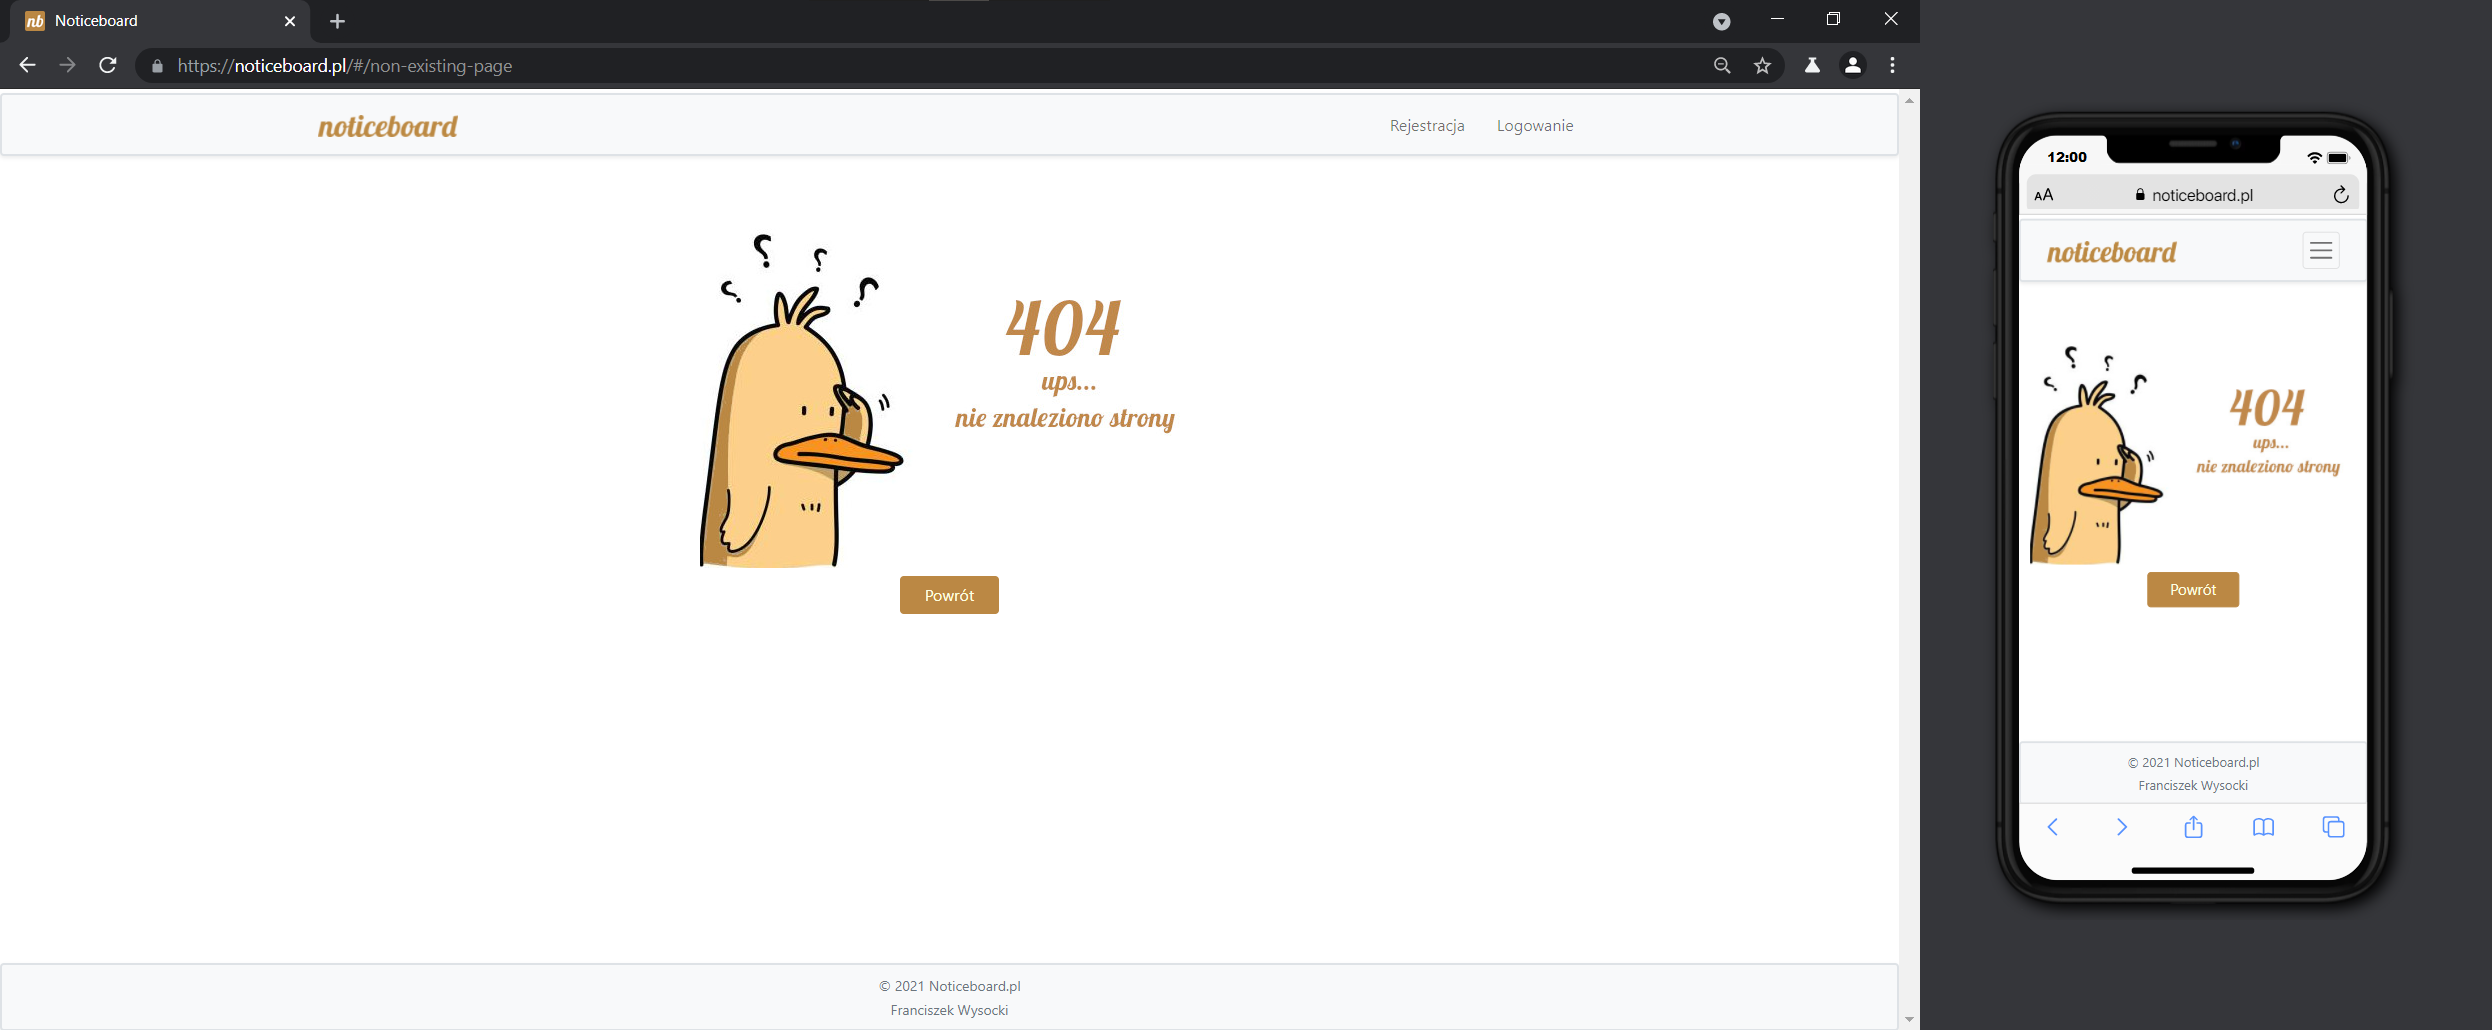
\includegraphics[width=15.5cm]{NieIstniejącaStrona.png}
                   \captionof{figure}{}
            \end{center}
        \item Użytkownik kilka w uszkodzony link aktywujący konto:
                    \begin{center}
                    \centering  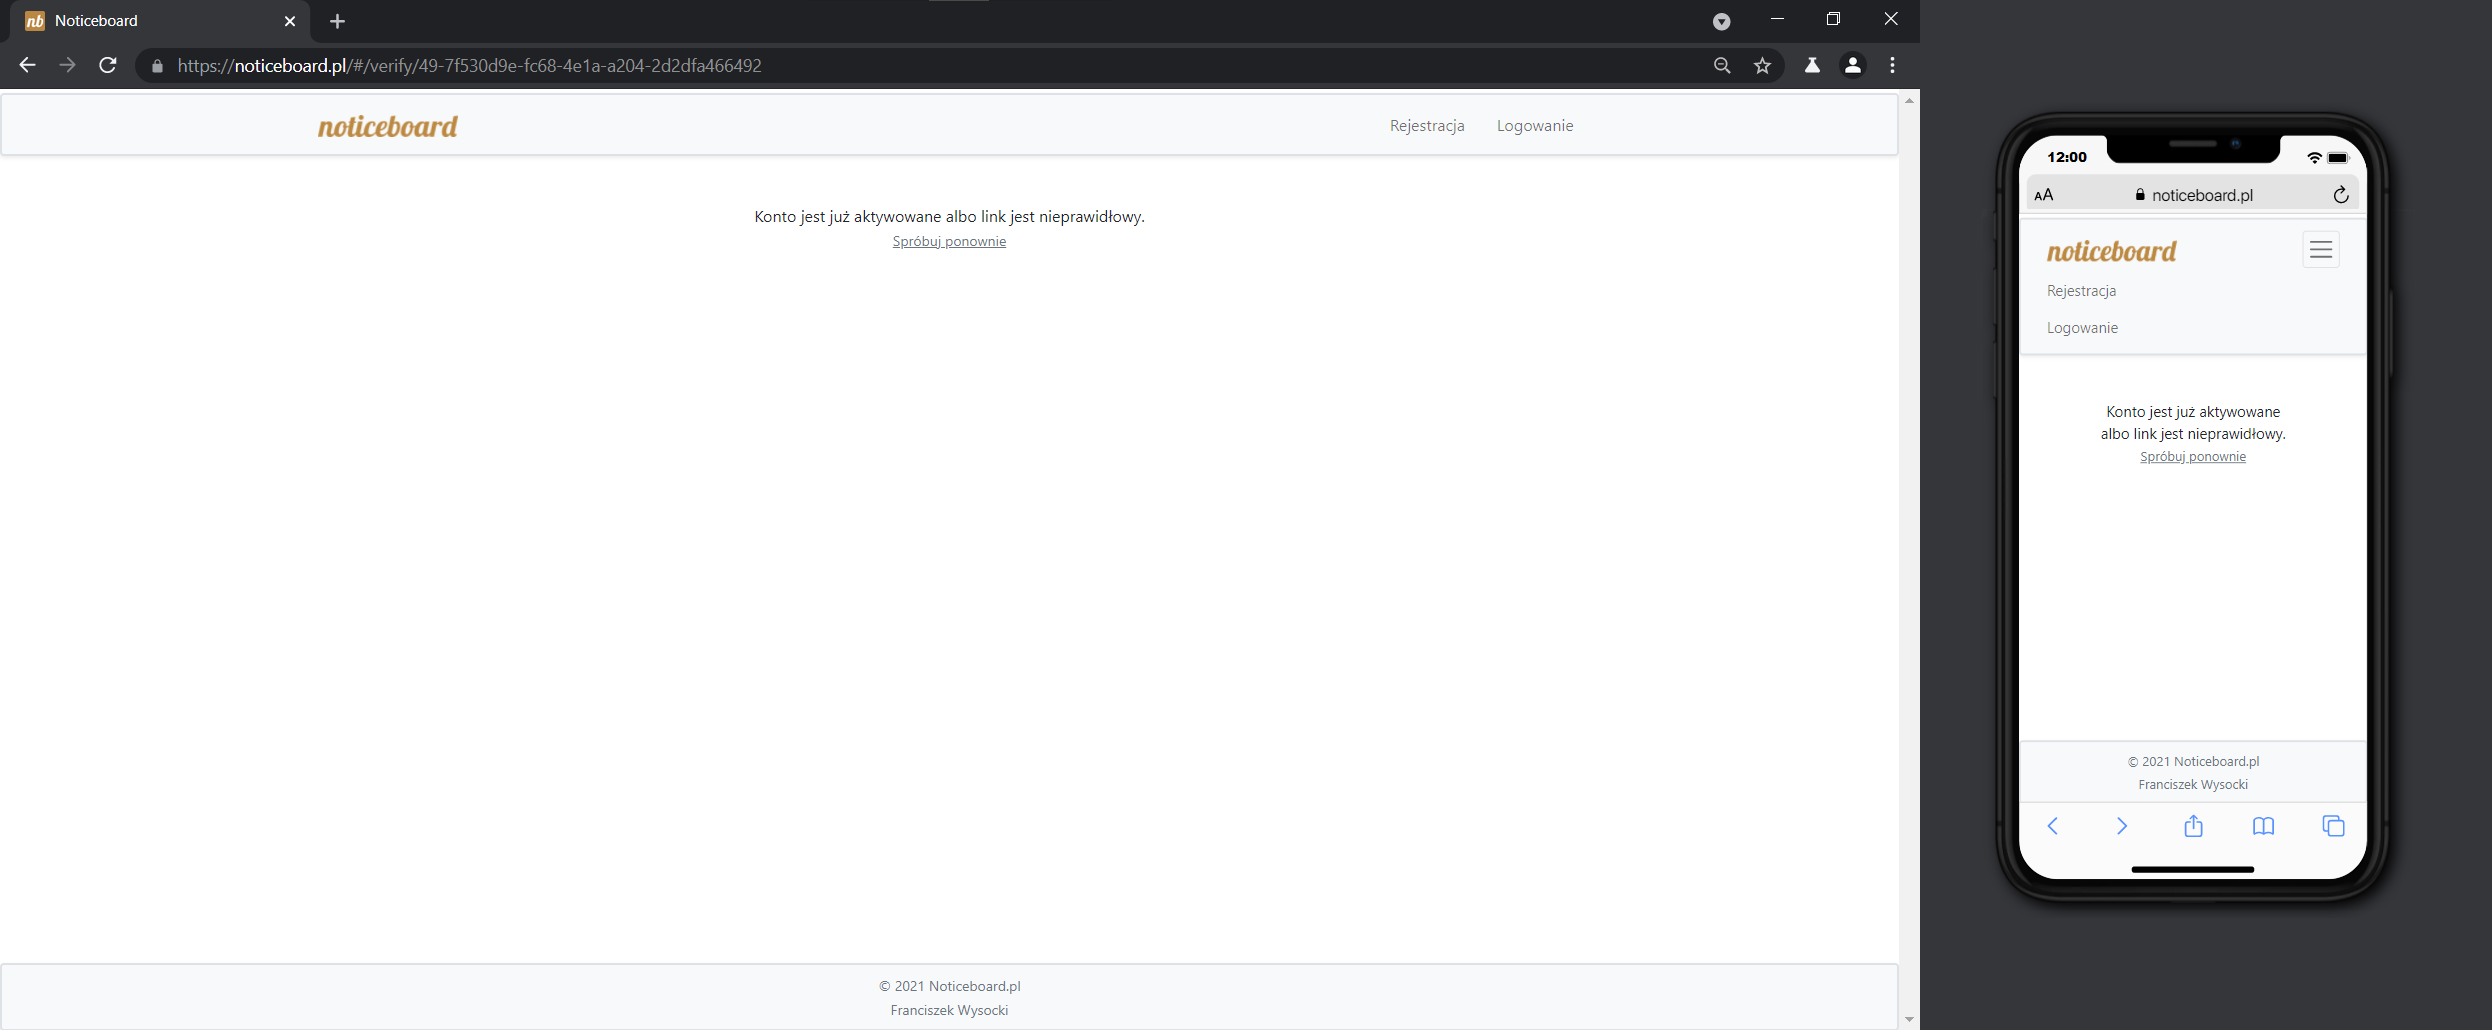
\includegraphics[width=15.5cm]{KlikniecieWNiepoprawnyLink.png}
                   \captionof{figure}{}
            \end{center}
        \item Użytkownik kilka w wygasły link aktywujący konto:
            \begin{center}
                    \centering  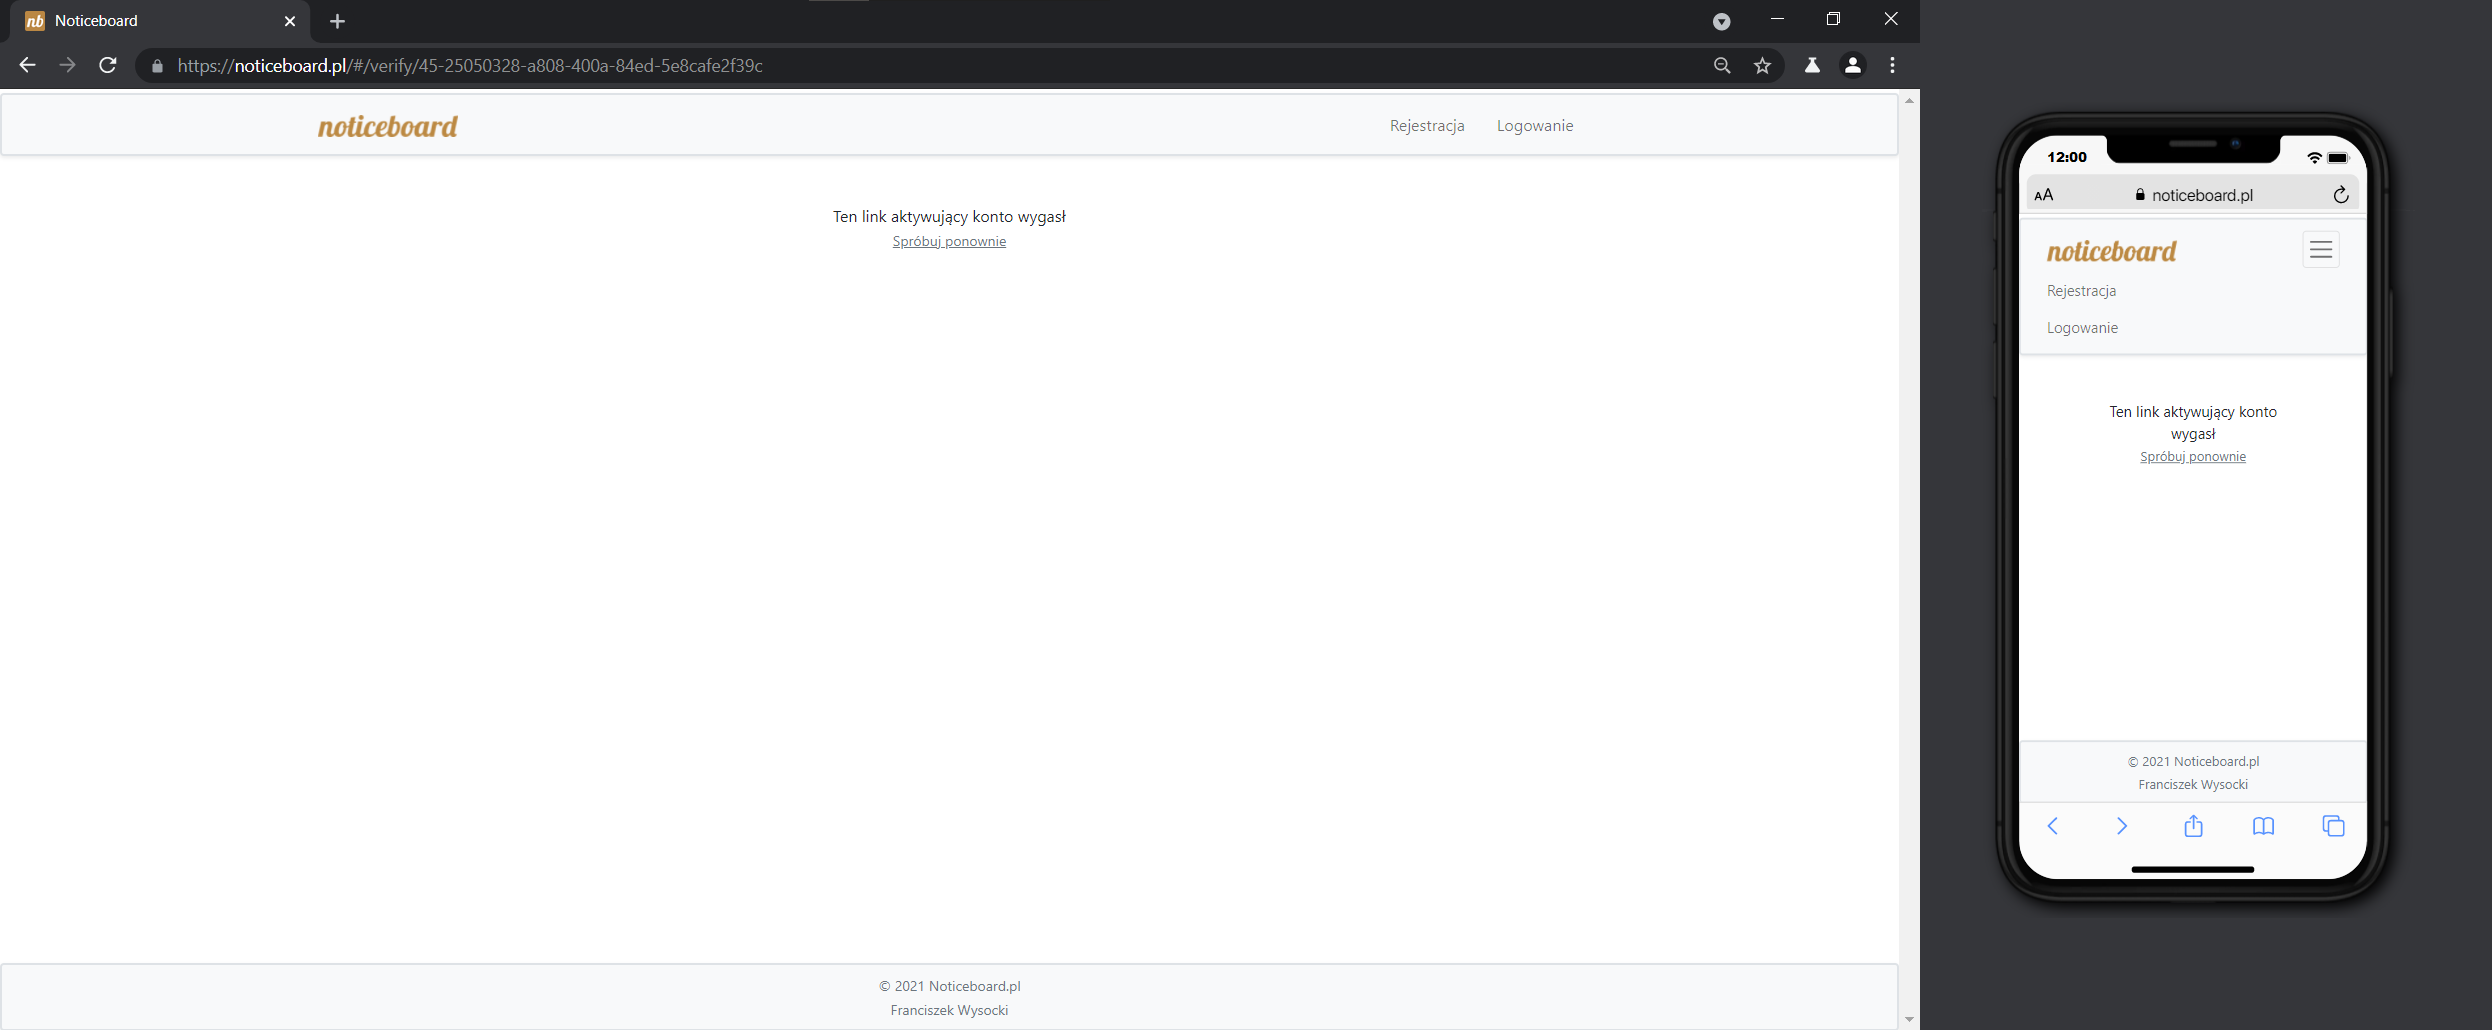
\includegraphics[width=15.5cm]{KliknięcieWWygaśniętyLink.png}
                   \captionof{figure}{}
            \end{center}
            
            
        Po kliknięciu ,,spróbuj ponownie'' użytkownik ma możliwość wysłania ponownego linku aktywacyjnego:
        \begin{center}
                    \centering  \includegraphics[width=15.5cm]{PonowneWysłanieLinku.png}
                   \captionof{figure}{}
        \end{center}
        \item Pozostałe obsługiwane błędy:
        \begin{itemize}
            \item Pozostawienie pustego pola w formularzu lub za krótki/długi ciąg znaków (komunikat);
            \item Niedopasowanie hasła/adresu e-mail do wzorca np. podczas rejestracji (komunikat); 
            \item Próba zalogowania, rejestracji, aktywacji konta, będąc zalogowanym (przekierowanie);
            \item Próba zarządzania czyimś ogłoszeniem/kontem (przekierowanie + zablokowanie po stronie back-endu).
        \end{itemize}
    \end{itemize}
    

    \lhead{Podsumowanie i wnioski}
    \section{Podsumowanie i wnioski}
         Największą przyjemność i jednocześnie największą trudność sprawiało mi implementowanie logiki aplikacji m.in. zarządzanie zdjęciami (od odczytu po serwowanie z cachowaniem), wysyłanie e-maili z tokenami (ważnymi 15 minut) i sam CRUD. Dużo czasu poświęciłem na samo wdrożenie aplikacji z certyfikatem SSL, co nie okazało się bardzo skomplikowane, ale brakowało mi wiedzy, jak to zrobić. 
         Bardzo spodobała mi się praca z Lombokiem, Mapstructem i Spring Data JPA, które pozwoliły na korzystanie z metod bez implementowania ich. \\
         
        Front-end aplikacji chciałem stworzyć prosty i elegancki. Starałem się też, aby aplikacja była responsywna i przetestowałem ją na kilku urządzeniach i przegladarkach. Praca nad front-endem była momentami uciążliwa np. przesuwanie się elementów po rozwinięciu panelu/filtrów, jednak udało mi się to wyeliminować. \\
        
        Sam projekt uważam za udany i jestem z niego bardzo zadowolony. Zrozumiałem i nauczyłem się bardzo wielu rzeczy, które myślę, że z pewnością wykorzystam w przyszłości.

\end{document}